\setcounter{chapter}{12-1} %Makes the prereq chapter chapter 0

\chapter{Markov Decision Processes 1 - Value Functions, Policies}

\setcounter{section}{0}

    We've developed a notion of a \vocab{state machine (SM)}: a system for keeping track of our \textit{current} situation, using a "state".

    \begin{itemize}
        \item This state also contains information about the \purp{past}: our \textbf{present} state is influenced by past data.
    \end{itemize}

    In particular, our focus is on \vocab{finite state machines}. \\

    \begin{clarification}
        For the rest of this chapter, we'll assume that our state machines are finite:

        \begin{itemize}
            \item Our set of \redd{states} and set of \brow{inputs} are finite.
        \end{itemize}
    \end{clarification}

    \begin{figure}[H]
        \centering
        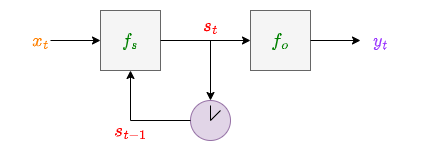
\includegraphics[width=80mm,scale=0.5]{images/rnn_images/state_machine_diagram.png}
        
        \caption*{A reminder of what our state machine looks like.}
    \end{figure}
    


    \phantom{}

    \subsection{A new perspective: the "outside world"}

        Now, we'll build on our state machine, to create something more specialized for what we need: this will require a new perspective.
        
        \begin{itemize}
            \item Our "state" has been referred to as our "current situation". This could suggest that it's \textbf{representing} something about the \gren{world}.
            
            \item In this perspective, our state machine is representing how the world \textbf{changes} over time.
            
            \item  In this case, the state of the world is what we're \textbf{interested} in: that's going to be our new \purp{output}.\\
        \end{itemize}

        \begin{concept}
            We can view the \gren{state} of our state machine as the current state of the \purp{outside world} that we're modeling.

            If we're interested in this "state" of our world, that is the \purp{output} we want:

            \begin{equation*}
                \pur{y_t} = \red{s_t}
            \end{equation*}

            \begin{itemize}
                \item $\grn{f_s}$ is the identity function $f_s(z)=z$: our state is returned, the same way it entered.
            \end{itemize}
            
        \end{concept}

        \miniex In a game, you might want to know \gren{where} you are: so, we keep track of "position" as a state, and return it as an output (on screen).

        \begin{figure}[H]
            \centering
            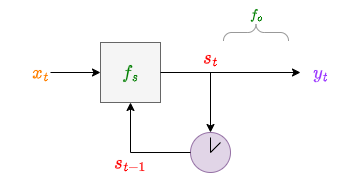
\includegraphics[width=80mm,scale=0.5]{images/mdp_images/state_machine_outputstate.png}
            
            \caption*{We can basically remove $f_o$: it has no effect.}
        \end{figure}



    \phantom{}

    \subsection{Making "decisions"}

        This is already interesting, but now, we'll build on this perspective:

        \begin{itemize}
            \item Often, we don't just want to simply \gren{observe} the world, we want to \brow{interact} with it.
            \item We might want to experiment with different ways to interact with, and change, our \orgg{model world}.
            \item Our state machine modifies its state ("world") through the \brow{input}. We'll use this input to interact with our world: we'll call it an \brow{action}.\\
        \end{itemize}

        \begin{concept}
            We want to be able to deliberately \purp{modify} the state of the \gren{outside world} though our interactions.

            \begin{itemize}
                \item With an SM, \purp{modify} the state of the world through our \brow{inputs}.
            \end{itemize}
            
            Thus, we'll replace our input $x_t$ with an \vocab{action} $a_t$.

            \begin{itemize}
                \item Our set of actions $\bro{\mathcal{A}}$ will replace $\bro{\mathcal{X}}$.
            \end{itemize}

        \end{concept}

        \begin{itemize}
            \item \miniex If you were playing a game, your actions might be "move up", "move down", "move left", or "move right".
            \item These would affect your \purp{position}, which we could encode in our state.
        \end{itemize}

        \begin{figure}[H]
            \centering
            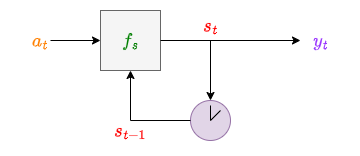
\includegraphics[width=80mm,scale=0.5]{images/mdp_images/action.png}
            
            \caption*{Structurally, nothing has really changed. $x_t$ has become $a_t$.}
        \end{figure}




    \phantom{}

    \subsection{Transitioning between States}

        One limitation of our state machines so far is that they're \vocab{deterministic}: the same inputs will always lead to the same outputs.\\

        \begin{definition}
            A \vocab{deterministic state machine} is one where the transitions between states are \purp{deterministic}: given the same inputs, we always get the same output.
        \end{definition}

        \begin{itemize}
            \item In a realistic setting, the same actions won't always have the same effect: we might end up with \purp{different} states, even if we take the same action.
        \end{itemize}

        Thus, we'll use \vocab{probabilistic} state transitions. Instead of outputting the same result every time, there will be a certain \gren{probability} of a given outcome.

        \miniex You have a plant you want to keep healthy. It's currently dry, so you choose the action "\brow{water}".

        \begin{itemize}
            \item 95\% of the time, the plant becomes "healthy": it's been watered, and has what it needs to grow.
            \item 5\% of the time, the plant becomes "sick": you just got unlucky, and the plant is sick now. 
                \note{Maybe you watered more than it needed, or maybe something about the environment changed... it doesn't really matter.}
        \end{itemize}

        This model doesn't require giving up on state machines: our function $f_s$ has just changed, returning a \purp{random variable}.\\

        \begin{concept}
            We want to be able to represent the \vocab{stochastic} (randomized) nature of our world.

            So, we include some randomness in our \gren{state transitions}: 

            \begin{itemize}
                \item Given a particular state $s_{t-1}$ and action $a_t$, \orgg{you don't know} exactly what state you'll get for $s_t$.
                \item Instead, we have a \purp{distribution}, which assigns a \gren{probability} to each possible next state.
            \end{itemize}

            We have a \vocab{probabilistic state machine}.
        \end{concept}

            \note{A probabilistic state machine is one type of "non-deterministic" state machine.}

        \begin{figure}[H]
            \centering
            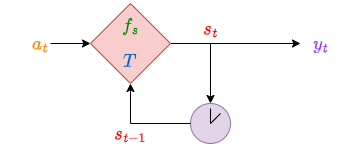
\includegraphics[width=80mm,scale=0.5]{images/mdp_images/transition_T.png}
            
            \caption*{$T$ represents the probability distribution of possible output states.}
        \end{figure}

        This kind of state machine is very similar to something called a \vocab{markov chain}.\\

        \begin{remark}
            Our \purp{probabilistic finite state machine (PFSM)} is roughly equivalent to an important mathematical model: a \vocab{markov chain}.

            In order to be a markov chain, however, it must fulfill the \vocab{Markov Property}:

            \begin{itemize}
                \item The state transition is \gren{memoryless}: it only depends on our most recent state $s_{t-1}$, not any earlier states.
            \end{itemize}

            This requirement is already met by our PFSM, but some more complex models may not.
        \end{remark}

            \note{This remark doesn't fully, rigorously define markov chains. However, we've already built a model that behaves very similarly.}

        The main difference from a markov chain is that, instead of having inputs, we have actions: a mechanism for making \textbf{decisions}.

        

    \pagebreak
    \subsection{Introducing Rewards}

        Fundamentally, all we've done so far is choose a particular type of state machine. But now, there's something we'd like to add:

        \begin{itemize}
            \item We have introduced the idea of an "action", but currently, we have reason to choose one action over another.
            \item To resolve this, we'll introduce an idea of which actions are "good": we'll give a \purp{reward} based on your state, and action.\\
        \end{itemize}

        \begin{concept}
            In addition to our markov chain/PFSM, we'll include a \vocab{reward function}, which tells us which situations are more or less desirable.

            This depends on both your \brow{action} and current \redd{state}. 
            
            \begin{itemize}
                \item These \vocab{state-action pairs} can be compared to each each other using the reward function.
            \end{itemize}
        \end{concept}

        \miniex A "reward" in a game might be represented by a change in your score.

        

        This reward creates two kinds of decision-making:\\

        \begin{concept}
            Our reward is determined by the \purp{state-action pair} it receives. This creates two different aspects that weigh into our decision:

            \begin{itemize}
                \item \gren{State}: how do we transition into the state(s) that give us the highest reward?
                \item \purp{Action}: which actions give us the highest reward?
            \end{itemize}

            Often, our model must choose between an action that moves you into a "more rewarding" \gren{state}, or an action that gives you higher \purp{immediate reward}.
        \end{concept}

        \miniex Do you spend your time getting the easy reward in one area, or try to go to a different, possibly more profitable area?

        Later, we'll introduce a \vocab{discount factor} $\gamma$, which influences this balance between immediate and long-term rewards.

        \begin{figure}[H]
            \centering
            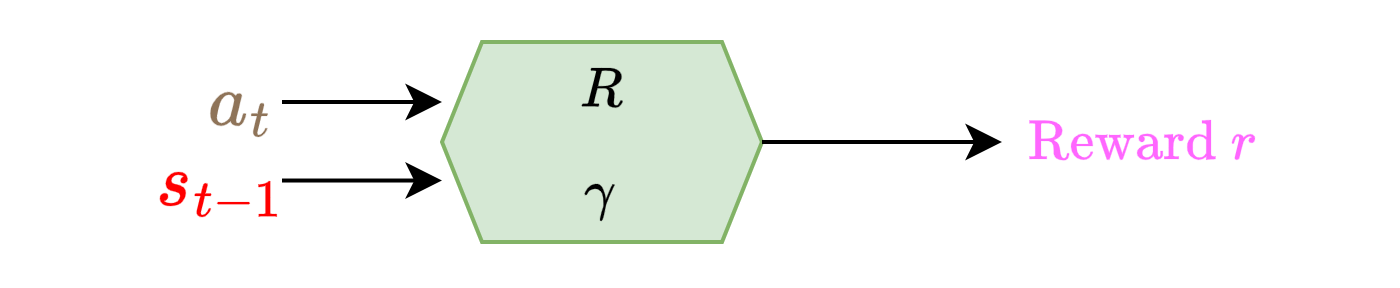
\includegraphics[width=80mm,scale=0.5]{images/mdp_images/reward_function.png}
            
            \caption*{$R$ is a function computing rewards, $\gamma$ is our discount factor we'll discuss later.}
        \end{figure}

        \begin{figure}[H]
            \centering
            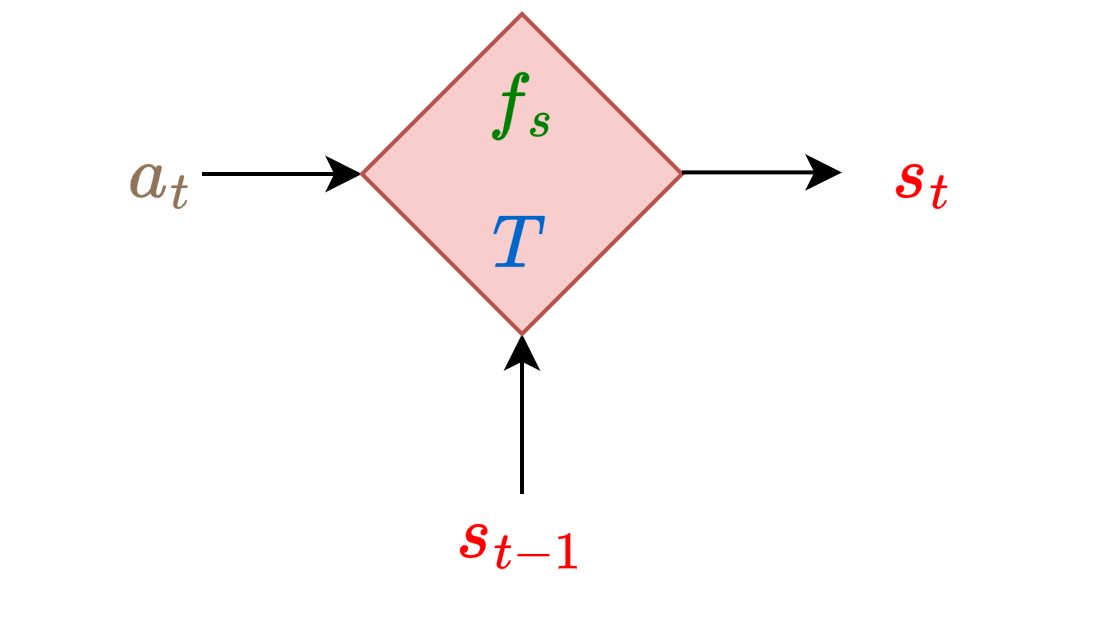
\includegraphics[width=60mm,scale=0.5]{images/mdp_images/state_machine_noloop.png}
            
            \caption*{We can compare to the state machine, if we ignore the circular component: they take the same inputs, with different outputs.}
        \end{figure}

        \begin{concept}
            Our \purp{reward function} and \gren{state machine} take the same inputs:

            \begin{itemize}
                \item The current state $s_{t-1}$
                \item The next action $a_t$
            \end{itemize}

            Based on this information, they tell us two different things:

            \begin{itemize}
                \item The \gren{state machine} tells us how this action affects the world, in this situation.
                \item The \purp{reward function} tells us how "good" this action is, in this situation.
                
            \end{itemize}

            The former tells us how the world has \orgg{changed}, while the latter tells us how \orgg{immediately} desirable this action was.
        \end{concept}

        Together, they give us a more complete understanding of this state-action pair.

        


        

        \pagebreak

    \subsection{Markov Decisions Processes}

        Taking all of these modifications together, we create a new model: the \vocab{Markov Decision Process}.\\

        \begin{definition}
            A \vocab{Markov Decision Process (MDP)} is a model building upon \orgg{state machines}.

            First, we make one labelling change:

            \begin{itemize}
                \item Our \brow{inputs} $x_t \in \mathcal{X}$ are replaced with \brow{actions} $a_t \in \mathcal{A}$.
            \end{itemize}

            \phantom{}

            Then, we select a particular variation of state machine:

            \begin{itemize}
                \item Our \redd{state} is returned as the \purp{output}: $\grn{f_o}(z) = z$
                    
                \item Our \orgg{transition} between states is now \purp{stochastic}: we have a certain probability of ending up in each new state.

            \end{itemize}

            \phantom{}

            Finally, we add one new structure outside the state machine:
            
            \begin{itemize}
                \item We include a \vocab{reward} function to evaluate the quality of these decisions, based on the \orgg{state-action} pair.
            \end{itemize}

        \end{definition}

        \phantom{}

        \begin{remark}
            Alternatively, we can view an MDP as a \vocab{markov chain}, with two modifications:

            \begin{itemize}
                \item \brow{Actions} replacing inputs, allowing for \purp{decisions}
                \item A \gren{reward function}, that allows us to evaluate those decisions.
            \end{itemize}
        \end{remark}

        Above, we depicted our state machine and our reward function separately. Here, we'll combine them:\\

        \begin{figure}[H]
            \centering
            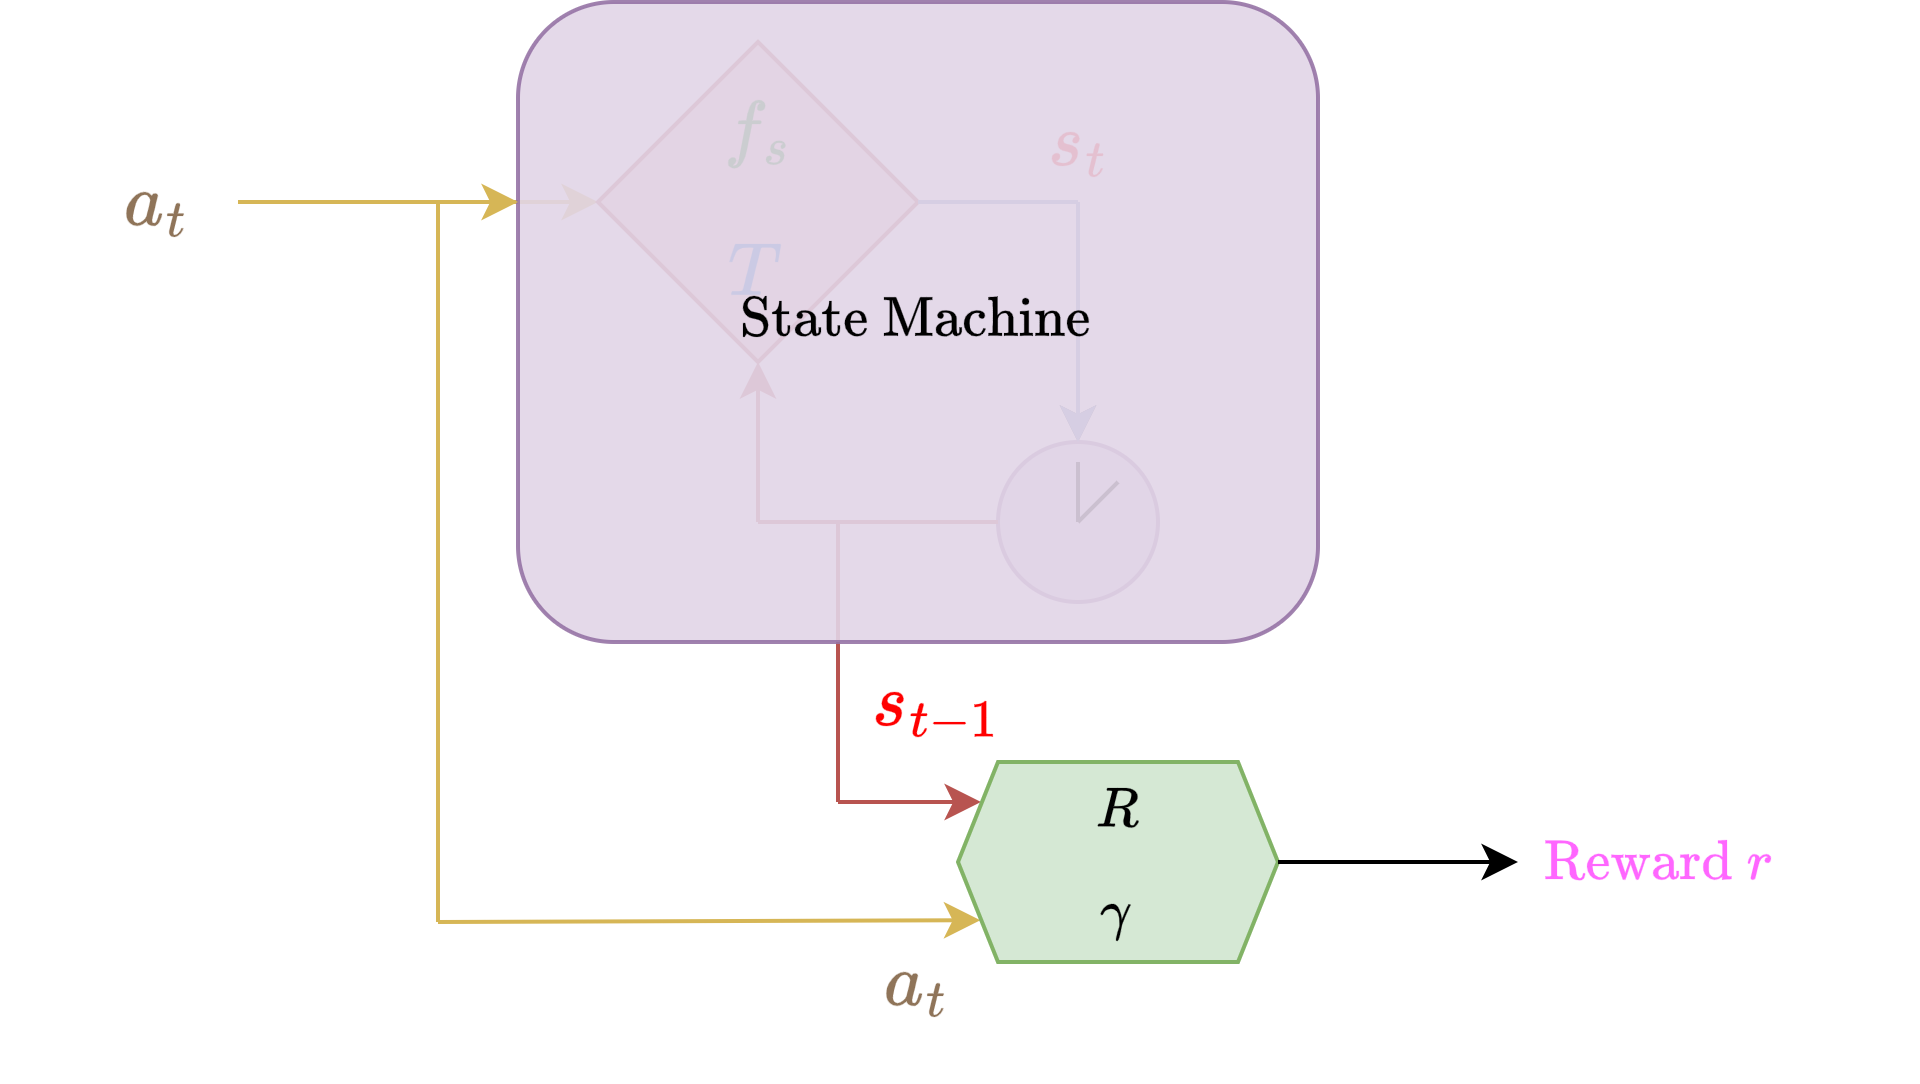
\includegraphics[width=120mm,scale=0.5]{images/mdp_images/mdp_opaque.png}
            
            \caption*{This represents our complete MDP, albeit simplified. We see our real goal: to figure out the relationship between action $a_t$, and our reward $r$.}
        \end{figure}

        \begin{figure}[H]
            \centering
            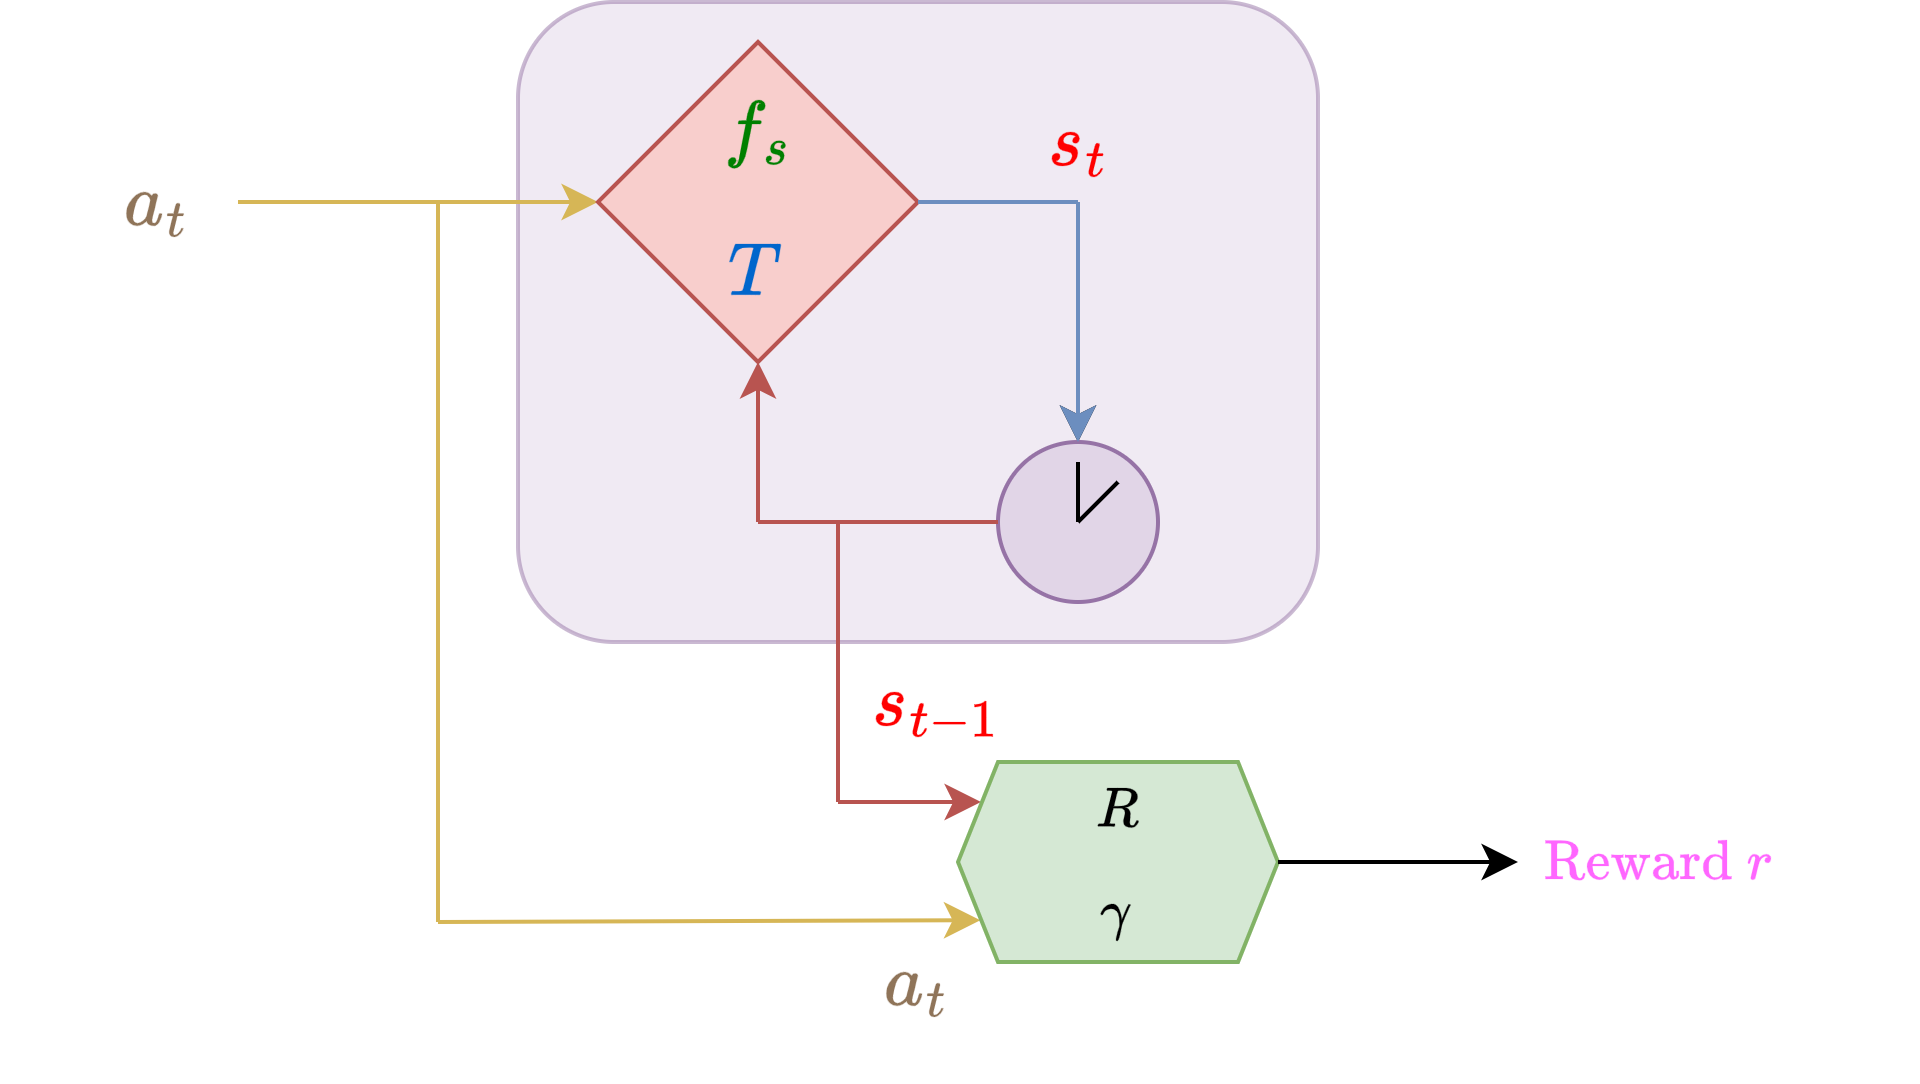
\includegraphics[width=120mm,scale=0.5]{images/mdp_images/mdp_transparent.png}
            
            \caption*{This view shows all the working parts: it's more complex, but more complete.}
        \end{figure}

        Our eventual goal is to find out how to \purp{maximize} our reward: we find out which actions provide the most reward.

        

    

        



\pagebreak
    
\section{Definition and Value Functions}

    \subsection{States and Actions in our MDP}

        We've laid out the general structure of our MDP, but now, we formalize each object.
    
        First, the familiar parts:\\
    
        \begin{definition}
            For our \vocab{MDP}, we have a \purp{finite} action space $\bro{\mathcal{A}}$ and state space $\red{\mathcal{S}}$.
    
            Thus, every action $a \in \mathcal{A}$, and every state $s \in \mathcal{S}$.
        \end{definition}
    
            \note{Remember: $a \in \mathcal{A}$ means "object $a$ is in the set $\mathcal{A}$.}

        \begin{itemize}
            \item Reminder that a "space" is just a set, with some extra structure.
                \note{The "structure" depends on what set we choose.}
            \item So, our action space is our set of actions, and our state space is our set of states.
        \end{itemize}


    \pagebreak            
    
    \subsection{Transition Model}
    
        Now, we need to represent the \purp{transition} between states.
    
        \begin{itemize}
            \item Each \textit{possible} state has a probability $p$ of being our \textit{next} state.
            \item We'll compute the probability with our \purp{transition model}.
        \end{itemize}
    
        Our transition model with give us a probability. But in order to know the probability, we need three piece of information:
    
        \begin{itemize}
            \item $\red{s}$: What is our current state? (Previously $s_{t-1}$)
    
            \item $\bro{a}$: What action did we take? (Previously $a_t$)
    
            \item $\pur{s'}$ What is the \gren{possible next state} we want to get the \purp{probability} of? (Possible $s_t$)
        \end{itemize}
    
        Our transition function $T$ takes these three pieces of information, and gives us the probability:

        \begin{equation}
            T(\red{s},\bro{a},\pur{s'}) \;\;=\;\; \text{Probability that, in \redd{state $s$}, \brow{action $a$} results in \purp{new state $s'$}}
        \end{equation}

        In more mathematical terms:
            \note{Because our state $S_t$ is now a random variable, we'll represent it with a capital letter.}

        \begin{equation}
            T(\red{s},\bro{a},\pur{s'}) \;\;=\;\; 
            \given{ \pur{S_t = s'}  }{\red{S_{t-1} = s},\quad \bro{A_t = a}}
        \end{equation}

        \begin{definition}
            The \vocab{transition function} $T$ gives the probability of 

            \begin{itemize}
                \item Entering state $\pur{s'}$,
                \item Given that we chose action $\bro{a}$ in state $\red{s}$
            \end{itemize}

            \begin{equation*}
                T(\red{s},\bro{a},\pur{s'}) \;\;=\;\; 
                \given{ \pur{S_t = s'}  }{\red{S_{t-1} = s},\quad \bro{A_t = a}}
            \end{equation*}

            After a transition, we will be in \orgg{exactly one} new state $s'$.

            \subsecdiv

            We can represent it using function notation by considering the following:

            \begin{itemize}
                \item $T$ has input (state, action, state): $\red{\mathcal{S}} \cross \bro{\mathcal{A}} \cross \pur{\mathcal{S}}$
                \item $T$ returns a probability: a real number between 0 and 1: $\Big[0, 1 \Big]$
            \end{itemize}

            \begin{equation*}
                T: \red{\mathcal{S}} \cross \bro{\mathcal{A}} \cross \pur{\mathcal{S}}
                \to \Big[0, 1 \Big]
            \end{equation*}
        \end{definition}

        It would also be valid to write $T: \red{\mathcal{S}} \cross \bro{\mathcal{A}} \cross \pur{\mathcal{S}}    \to \RR$, because $\Big[0, 1 \Big]$ is part of the real numbers $\RR$.

        \miniex We'll return to the example of our plant. 
        
        \begin{itemize}
            \item Its current state is $\red{s}=\text{Dry}$.
            \item We choose action $\bro{a}=\text{Water}$.
        \end{itemize}

        We have two outcomes:

        \begin{itemize}
            \item 95\% chance of becoming healthy.
                \begin{equation}
                    T \Big( 
                        \text{\red{Dry}}, \text{\bro{Water}}, \text{\pur{Healthy}} 
                      \Big)
                   = 0.95
                \end{equation}

            \item 5\% chance of becoming sick.
                \begin{equation}
                    T \Big(
                        \text{\redd{Dry}}, \text{\bro{Water}}, \text{\grn{Sick}} 
                      \Big)
                    = 0.05
                \end{equation}
                
        \end{itemize}


    
    \phantom{}

    \subsection{Comments on our Transition Function}

        Note that we said that we transition to \textbf{exactly one} new state. This means two things:

        \begin{itemize}
            \item Each new state $s'$ is \purp{disjoint}.
            \item We will definitely end up in \gren{one} of those sets.
        \end{itemize}

        Combined, we can say that the probability of all of our states $s'$ adds to 1.\\

        \begin{concept}
            Given a particular \redd{state $s$} and \brow{action $a$}, the probabilities for all new sets \gren{s'} adds to 1:

            \begin{equation*}
                \sum_{ \pur{s' \in \mathcal{S}} } T \Big(\red{s},\bro{a},\pur{s'} \Big) = 1
            \end{equation*}

            
        \end{concept}

        \subsecdiv

        One more comment: we use our transition to determine the probability of state transitions.

        However, $T$ is \redd{not} our state transition function $f_s$.\\

        \begin{clarification}
            While $T$ and $f_s$ are both involved in \vocab{state transitions}, they serve different functions:

            \begin{itemize}
                \item $T$ gives the \purp{probability} of entering a new state, based on our old states.
                
                \item $f_s$ actually \gren{gives us} the new state, according to those probabilities.
                
            \end{itemize}

            In other words, $T$ is a function which \orgg{describes} how $f_s$ behaves.
        \end{clarification}

        They even have different inputs/output sets:

        \begin{equation}
            \begin{matrix}
                T: \red{\mathcal{S}} \cross \bro{\mathcal{A}} \cross \pur{\mathcal{S}}   \to \Big[0, 1 \Big] && 
                f_s: \red{\mathcal{S}} \cross \bro{\mathcal{A}}  \to \pur{\mathcal{S}}\\\\
                T\Big( \red{s},\bro{a},\pur{s'} \Big)= p && f_s\Big(\red{s},\bro{a}\Big)=\pur{s'}
            \end{matrix}
        \end{equation}



    \phantom{}

    \subsection{State-Transition Diagram: Review}

        Our state-transition diagram needs an upgrade, now that our transitions can be probabilistic.

        First, we'll review our example from the \vocab{RNN chapter}.

        \miniex We have a blanket. It can be in three states: either \blu{wet}, \grn{dry}, or \red{burning}. We can represent each state as a "node".

        \begin{itemize}
            \item To change its state, we can either add "water" or "fire".
        \end{itemize}
        
        \begin{figure}[H]
            \centering
            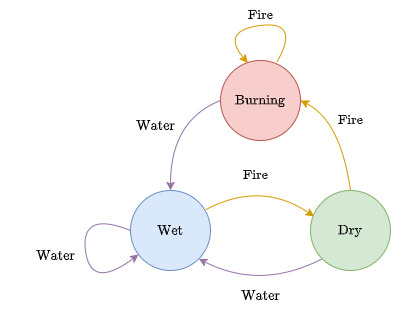
\includegraphics[width=80mm,scale=0.4]{images/rnn_images/std_fire_and_water.png}
        \end{figure}

        We want to update this to include transition probabilities.
        
        \begin{itemize}
            \item But this would get pretty dense and \textbf{complex}: each arrow would require a \redd{state}, and a \gren{probability}.
            \item Even worse: right now, we only have one possible outcome for each state-action pair.
                \begin{itemize}
                    \item But our probabilistic version allows for multiple outcomes: more arrows, more complexity.
                        \note{There could be 2 or more outcomes in the same situation, based on probability.}
                \end{itemize}
                    
        \end{itemize}

        So, we'll split up our diagram based on the \brow{action}, like we did in the RNN chapter:
        
        \begin{figure}[H]
            \centering
            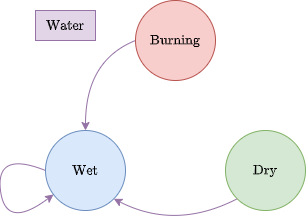
\includegraphics[width=60mm,scale=0.4]{images/rnn_images/std_water_no_label.png}
            \qquad
            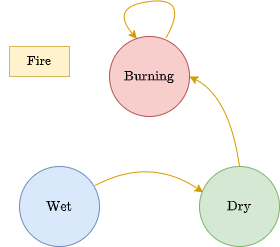
\includegraphics[width=55mm,scale=0.4]{images/rnn_images/std_fire.png}
            
            \caption*{The left diagram uses \textbf{water} as an input, while the right diagram uses \textbf{fire} as an input.}
        \end{figure}



    \phantom{}

    \subsection{State-Transition Diagram: Probabilistic}

        Now, we can extend these diagrams with probabilities.

       We'll use the following:

        \begin{itemize}
            \item Add water
                \begin{itemize}
                    \item \redd{Burning} blanket: \grn{30\%} dry, \blu{50\%} wet, \red{20\%} burn.
                    \item \vocab{Wet} blanket: \blu{100\%} wet.
                    \item \gren{Dry} blanket: \grn{10\%} dry, \blu{90\%} wet.
                \end{itemize}

                \begin{figure}[H]
                    \centering
                    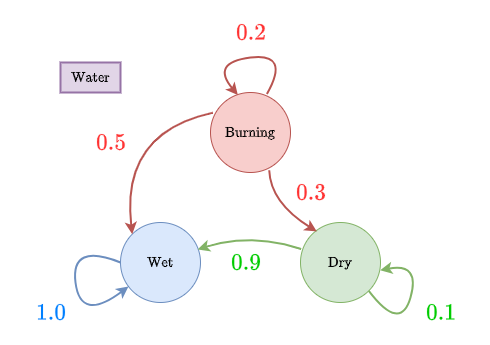
\includegraphics[width=80mm,scale=0.4]{images/mdp_images/add_water_transition.png}
                \end{figure}
        \end{itemize}

        \begin{itemize}
            \item Add fire
                \begin{itemize}
                    \item \redd{Burning} blanket: \grn{10\%} dry, \red{90\%} burn.
                    \item \vocab{Wet} blanket: \grn{50\%} dry, \blu{40\%} wet, \red{10\%} burn.
                    \item \gren{Dry} blanket: \grn{20\%} dry, \red{80\%}  burn.
                \end{itemize}

                \begin{figure}[H]
                    \centering
                    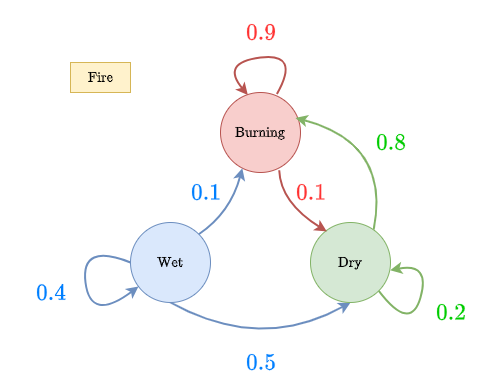
\includegraphics[width=80mm,scale=0.4]{images/mdp_images/add_fire_transition.png}
                \end{figure}
        \end{itemize}

        These would be almost impossible to represent in a readable way if we include every action on the same graph. So, we create a separate graph for each action.
        
        \begin{itemize}
            \item If we add more actions, our graph becomes no more complex: we just create more graphs.\\
        \end{itemize}

        \begin{concept}
            For MDPs, we usually have a separate \vocab{state-transition diagram} for each \brow{action}.
        \end{concept}

        A second comment: Notice that, when adding water to a wet blanket, it has a 100\% chance to stay wet.

        \begin{itemize}
            \item This example is \gren{equivalent} to the deterministic state machine from the RNN chapter: based on our state and action, we know exactly what state we end up with next.\\
        \end{itemize}

        

        \begin{concept}
            Our \vocab{MDP} can reproduce a \purp{deterministic} state machine by setting the probability for every outcome to 0 or 1.
        \end{concept}

            \note{Of course, we still need 1 valid action for each state-action pair.}




    \phantom{}

    \subsection{Transition Matrix}

       Representing our transitions is made complicated by the fact that we have three parameters: $T(\red{s},\bro{a},\pur{s'}) $.

       \begin{itemize}
           \item If we wanted to represent the outputs, with each parameter on one axis, we'd need a 3-tensor to depict the whole thing.
       \end{itemize}

       But above, for graphing purposes, we found a solution: separating our transitions based on our \brow{action $a$}.

       \begin{itemize}
           \item If we only consider one action $\bro{a}$, we only have two parameters: $\red{s}$ and $\pur{s'}$.
           \item We can represent this with a \textbf{matrix} $\mathcal{T}$.
       \end{itemize}

       One axis will indicate the previous state $\red{s}$, and the other axis will represent the new state $\pur{s'}$.
       
        \begin{itemize}
            \item We'll use rows for $\red{s}$ (input state), and columns for $\pur{s'}$ (output state).

            \begin{equation}
                \mathcal{T}(\bro{a}) 
                \quad = \quad
                \begin{matrix}
                    \text{Input } \text{state} \\ \red{s}
                \end{matrix}
                \mathlarger{\Bigg\{}
                \overbrace{
                    \begin{bmatrix}
                        ? & ? & ? \\
                        ? & ? & ? \\
                        ? & ? & ?
                    \end{bmatrix}
                    }^{\text{ \small Output state $\pur{s'}$}}
            \end{equation}
            
            \item The element in our matrix will represent the \orgg{probability} of this transition.

            \begin{equation}
                \mathcal{T}(\bro{a})_{ij} = 
                T \Big( \red{s_i}, \bro{a}, \pur{s_j} \Big)
            \end{equation}
        \end{itemize}

        \begin{notation}
            One way to represent our \vocab{transition $T$} is to create a separate \purp{matrix} $\mathcal{T}$ for each action $\bro{a}$ where

            \begin{itemize}
                \item Row $i$ starts in state $s_i$
                \item Column $j$ moves us to state $s_j$
            \end{itemize}

            In this cell, we have:

            \begin{equation*}
                \mathcal{T}(\bro{a})_{ij} = 
                T \Big( \red{s_i}, \bro{a}, \pur{s_j} \Big)
            \end{equation*}
            
            \begin{itemize}
                \item The probability that, in state $\red{s_i}$, action $\bro{a}$ takes us to state $\pur{s_j}$.
            \end{itemize}
        \end{notation}

        \miniex Suppose we have 3 states: $\red{s_1}$, $\grn{s_2}$, $\blu{s_3}$. Our matrix for action $a$ looks like:

        \begin{equation}
            \mathcal{T}(a) \quad = \quad 
            \begin{bmatrix}
                T \Big( \red{s_1}, a, \red{s_1}  \Big)& 
                T \Big( \red{s_1}, a, \grn{s_2}  \Big)&
                T \Big( \red{s_1}, a, \blu{s_3}  \Big)\\
                T \Big( \grn{s_2}, a, \red{s_1}  \Big)&    
                T \Big( \grn{s_2}, a, \grn{s_2}  \Big)&
                T \Big( \grn{s_2}, a, \blu{s_3}  \Big)\\
                T \Big( \blu{s_3}, a, \red{s_1}  \Big)&
                T \Big( \blu{s_3}, a, \grn{s_2}  \Big)&
                T \Big( \blu{s_3}, a, \blu{s_3}  \Big)
            \end{bmatrix}
        \end{equation}

        We'll practice on our usual blanket example. We label each of our states with an index:

        \begin{equation}
            \begin{bmatrix}
                s_1 \\ s_2 \\ s_3
            \end{bmatrix}
            = 
            \begin{bmatrix}
                \text{Burning} \\ \text{Dry} \\ \text{Wet}
            \end{bmatrix}
        \end{equation}

        With this, we can create a matrix for each action.

        \begin{figure}[H]
            \centering
            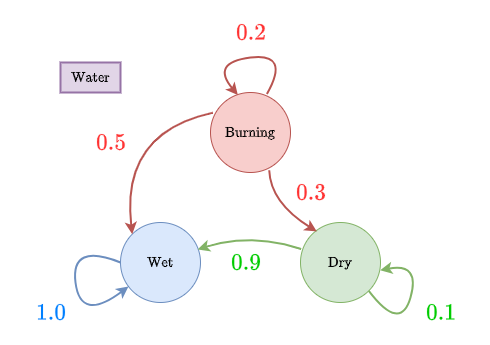
\includegraphics[width=80mm,scale=0.4]{images/mdp_images/add_water_transition.png}
        \end{figure}

        \begin{equation}
            \mathcal{T}(\blu{Water}) = 
                \begin{bmatrix}
                \red{0.2} & \red{0.3} & \red{0.5} \\
                \grn{0} & \grn{0.1} & \grn{0.9} \\
                \blu{0} & \blu{0} & \blu{1.0}
            \end{bmatrix}
        \end{equation}

        \begin{figure}[H]
            \centering
            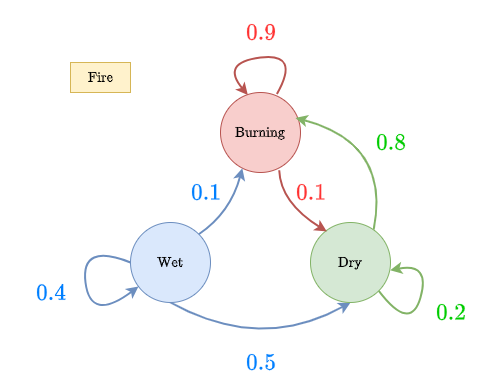
\includegraphics[width=80mm,scale=0.4]{images/mdp_images/add_fire_transition.png}
        \end{figure}

        \begin{equation}
            \mathcal{T}(\red{Fire}) = 
                \begin{bmatrix}
                \red{0.9} & \red{0.1} & \red{0} \\
                \grn{0.8} & \grn{0.2} & \grn{0} \\
                \blu{0.1} & \blu{0.5} & \blu{0.4}
            \end{bmatrix}
        \end{equation}

    \pagebreak

    \subsection{Reward Function}

        We'll represent our \purp{reward function}:

        \begin{itemize}
            \item We compute the \gren{reward} of each state-action pair as with a number: $r \in \RR$.\\
        \end{itemize}

        \begin{definition}
            Our \vocab{reward function} $R$ gives the \purp{reward} of a particular \redd{state}-\brow{action} pair.

            This indicates how desirable it is to 

            \begin{itemize}
                \item Choose action $\bro{a}$
                \item From state $\red{s}$
            \end{itemize}

            \begin{equation*}
                \pur{R} \Big( \red{s},\bro{a} \Big)  = r
            \end{equation*}

            \subsecdiv

            We determine our function notation by analyzing the input/output pair.

            \begin{itemize}
                \item $R$ has input (state, action): $\red{\mathcal{S}} \cross \bro{\mathcal{A}}$
                \item $R$ returns a "reward" as a real number: $\pur{R} \Big( \red{s},\bro{a} \Big) \in \RR$.
            \end{itemize}

            \begin{equation*}
                R: \red{\mathcal{S}} \cross \bro{\mathcal{A}} \to \RR
            \end{equation*}
        \end{definition}

        \miniex In our blanket example, we may only care about the state, not the action.
            \note{Maybe we're trying to use the blanket. A dry blanket can be used, a wet blanket cannot, and a burning blanket is an active problem.}

        \begin{equation}
            \pur{R} \Big( \red{s},\bro{a} \Big) =
            \begin{cases}
                10 & \red{s} = \text{Dry} \\
                0 & \red{s} = \text{Wet} \\
                -20 & \red{s} = \text{Burning}
            \end{cases}
        \end{equation}

        \begin{concept}
            Sometimes, our \vocab{reward function} may only depend on the \purp{state} we are in. 

            For consistency, we still use the notation $\pur{R} \Big( \red{s},\bro{a} \Big)$.
        \end{concept}

        One thing to be careful of:\\

        We'll procrastinate the discussion of our discount factor $\gamma$ to our discussion of \textbf{infinite horizon}.
            \note{In the meantime, we'll include it in our formal definition, but we won't discuss it.}


    \pagebreak

    

    \subsection{MDP Formalized}

        Finally, we've built all the pieces we need for a mathematical definition of our MDP.\\

        \begin{definition}
            We formally define \vocab{Markov Decision Process (MDP)} as a list of 5 objects: $\Big( \red{\mathcal{S}}, \bro{\mathcal{A}}, \grn{T}, \pur{R}, \pur{\gamma} \Big)$

            \begin{itemize}
                \item $\red{\mathcal{S}}$ is our \redd{state space}, and $\bro{\mathcal{A}}$ is our \brow{action space}.

                \begin{equation*}
                    \red{s \in \mathcal{S}}  \qquad \qquad \bro{a \in \mathcal{A}}
                \end{equation*}

                \item $\grn{T} \Big( \red{s},\bro{a},\pur{s'} \Big)$ is our \gren{transition function}, which gives us the \textbf{probability} of transitioning from state $\red{s}$ to state $\pur{s'}$, if we take action $\bro{a}$.

                \begin{equation*}
                    \begin{gathered}
                        T: \red{\mathcal{S}} \cross \bro{\mathcal{A}} \cross \pur{\mathcal{S}}   \to \Big[0, 1 \Big]\\
                    \end{gathered}           
                \end{equation*}

                \begin{equation*}
                    T(\red{s},\bro{a},\pur{s'}) \;\;=\;\; 
                    \given{ \pur{S_t = s'}  }{\red{S_{t-1} = s},\quad \bro{A_t = a}}
                \end{equation*}

                \item $\pur{R} \Big( \red{s},\bro{a} \Big)$ is our \purp{reward function}, which tells how \textbf{desirable} a particular state-action pair is.

                \begin{equation*}
                    R: \red{\mathcal{S}} \cross \bro{\mathcal{A}} \to \RR
                \end{equation*}
    
            \end{itemize}
            
            

        \end{definition}

        Lastly, we have our discount factor:
            \note{Some definitions treat the discount factor as separate from the MDP. We do not.}\\

        \begin{definition}
            $\pur{\gamma}$ is our \purp{discount factor}, which tells us how much we value future rewards.

            \begin{equation*}
                \gamma \in \Big[ 0,1 \Big]
            \end{equation*}

            The \gren{higher} $\gamma$ is, the \gren{more} we value future rewards.

            \begin{itemize}
                \item A reward $t$ timesteps in the future, is worth $\gamma^t$ times as much.
            \end{itemize}

            \subsecdiv

            Because $\gamma$ is never larger than 1, our discount factor can only:

            \begin{itemize}
                \item Treat future rewards as \purp{equal} to current rewards ($\gamma=1$) or

                \item Treat future rewards as \purp{lesser} than current rewards ($\gamma<1$)
            \end{itemize}
        \end{definition}

    \pagebreak

    

    \subsection{Policies}

        We've discussed taking \brow{actions $a$}: these are the \purp{decisions} we want to model with our MDP.

        \begin{itemize}
            \item But we haven't actually created a model for \gren{choosing} these actions.
        \end{itemize}

        At best, we could select a \orgg{sequence} of actions, and then see what reward we get on average. That way, we can compare them.
            \note{This strategy is based on our "sequence of inputs" from the RNN chapter.}

        \begin{equation}
            \begin{bmatrix}
                a_1 & a_2 & \cdots & a_n
            \end{bmatrix}
        \end{equation}

        But this approach doesn't make use of the \purp{current state}:
    
        \begin{itemize}
            \item In an MDP, our state transitions are \gren{stochastic}: we don't know exactly what the next state is going to be. 
            \item Based on what state we get, the "best" sequence would change.\\
        \end{itemize}

        \begin{concept}
            One weakness of using a pre-planned sequence of actions is that our model is \gren{stochastic}:

            \begin{itemize}
                \item Depending on how our state \purp{randomly} changes, the "best next action" changes.
            \end{itemize}
        \end{concept}

        \miniex Imagine we model poker as an MDP. If you used the \gren{exact same strategy} every time, while ignoring your cards (your "state"), you'd be a pretty terrible player.

        It would be better if we could \orgg{adapt} our choice of \brow{action}, based on the \redd{state} we ended up in.

        We'll construct a new function that does just that, called a \vocab{policy} $\pi$.\\

        \begin{definition}
            Our \vocab{policy} $\pi$ is a function used to compute \brow{our next action} based on our \redd{current state}.

            \begin{equation*}
                \pi \big(\red{s}\big) = \bro{a}
            \end{equation*}

            One policy represents one particular \orgg{strategy} for interacting with the MDP.

            \begin{equation*}
                \pi: \red{\mathcal{S}} \to \bro{\mathcal{A}}
            \end{equation*}

            \begin{figure}[H]
                \centering
                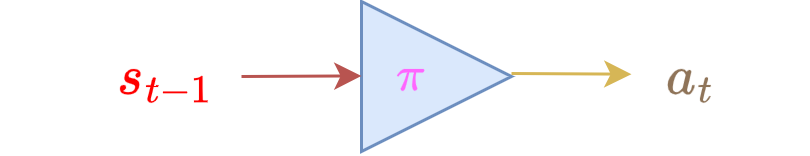
\includegraphics[width=60mm,scale=0.5]{images/mdp_images/policy.png}
            \end{figure}
        \end{definition}

        \miniex Here's one possible policy for our blanket example.
            \note{To be fair, we should probably add a third action that is neither "add water", nor "add fire". But this is an example policy: it isn't necessary the best policy.}

        \begin{equation}
            \pi \big( \red{s} \big) =
            \begin{cases}
                \text{\brow{Add fire}} & s = \red{Wet} \\
                \text{\brow{Add water}} & s = \red{Dry} \\
                \text{\brow{Add water}} & s = \red{Burning}
            \end{cases}
        \end{equation}

        

        This system allows our policy to "react" to changes in our state.
        
        \begin{itemize}
            \item If we run our MDP twice, and our state changes are \redd{different}, our \purp{policy} will choose different actions accordingly.
            \item \miniex In our poker example, our policy chooses actions based on the cards in your hand, and on the table.
        \end{itemize}


        Note that a policy $\pi$ is not necessary \purp{optimal}:\\

        \begin{clarification}
            As long as you provide an \brow{action} for every \redd{state}, you have created a valid \purp{policy}.

            \begin{itemize}
                \item This means that a policy doesn't have to make sense, or even be a \gren{good} policy.
            \end{itemize}

            Which policy is "good" depends on entirely on our \vocab{reward function}.
        \end{clarification}

        \miniex Here's our "pyromaniac" policy. This is probably not optimal unless you really like setting things on fire.
            \note{But it could be, depending on the reward function.}

        \begin{equation}
            \pi_p \big(\red{s} \big) =
            \begin{cases}
                \text{\brow{Add fire}} & s = \red{Wet} \\
                \text{\brow{Add fire}} & s = \red{Dry} \\
                \text{\brow{Add fire}} & s = \red{Burning}
            \end{cases}
        \end{equation}

        \subsecdiv

        Our policy is used by our MDP to process through time, generating actions.

        \begin{itemize}
            \item So, let's add it to our MDP diagram.
        \end{itemize}

        \begin{figure}[H]
            \centering
            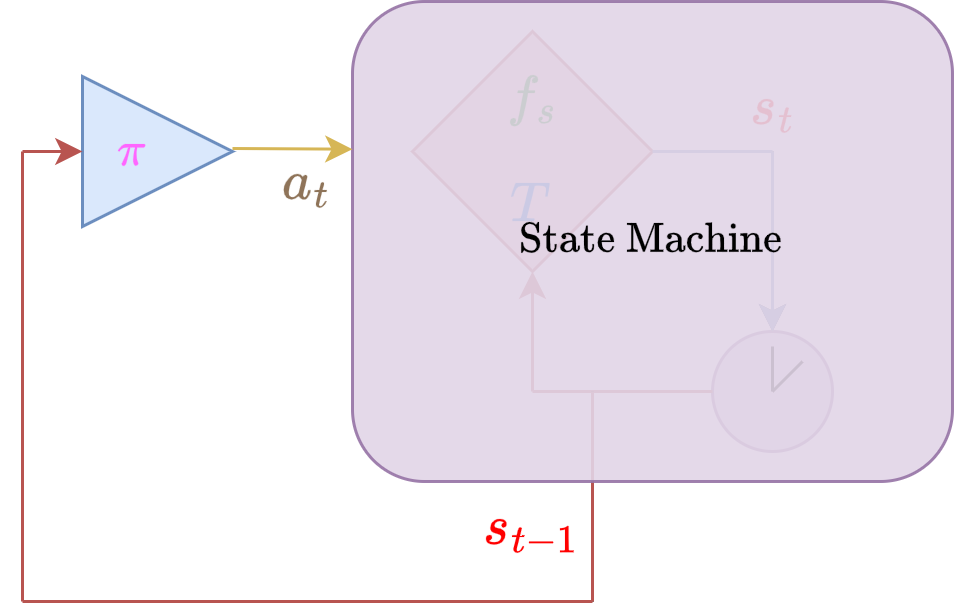
\includegraphics[width=70mm,scale=0.5]{images/mdp_images/policy_statemachine.png}
            
            \caption*{Our policy chooses an action based on the state, and the state machine answers with our new state. And so, the cycle continues.}
        \end{figure}
        

        In the coming sections, we'll consider two different kinds of problems for our "game" (MDP):

        \begin{itemize}
            \item Finite horizon -- we have exactly $T$ timesteps remaining before we finish our "game".
            \item Infinite horizon -- we have no upper limit on when the "game" ends.
                \note{But it might end eventually.}
        \end{itemize}


    \pagebreak

    \subsection{Value Functions}

        We've built up our MDP, a model to help us making \purp{decisions}. Now, we want the \gren{best policy}.\\

        \begin{concept}
            Typically, the \vocab{optimal policy} is the one that gives us the \gren{highest rewards}, on average.

            \begin{itemize}
                \item Averaged over our \purp{stochastic}, random state transitions.
            \end{itemize}
        \end{concept}

        Now, we need a way to directly \purp{compute} this average reward, for each policy: that way, we can compare them.

        We'll create a function for this purpose. It'll depend on two things:

        \begin{itemize}
            \item Our chosen \gren{policy}
            \item Our current \redd{state}
                \note{Different states earn \textbf{different} rewards, even with the \textbf{same} policy: 
                
                \phantom{}
                
                A perfect robot (same policy) could do better in the stock market if they had \textbf{more money} (different state).}
        \end{itemize}

        With this information, we'll compute the average reward: this represents the worth of our policy, so we call it our \vocab{value function}.\\

        \begin{definition}
            A \vocab{value function} $V_{\grn{\pi}}\big(\red{s} \big)$ gives us the \purp{average reward} of our policy $\grn{\pi}$, starting from state $\red{s}$.

            This allows us to compute which policies are "\gren{more valuable}" in a particular \redd{state}.

            \begin{itemize}
                \item Let's use \orgg{function} notation. Reward $r \in \RR$ is a real number. So, the same is true for our average reward $V_{\grn{\pi}}\big(\red{s} \big)$.
            \end{itemize}

            \begin{equation*}
                V_{\grn{\pi}}:  \red{\mathcal{S}} \to \pur{\RR}
            \end{equation*}

        \end{definition}

        \subsecdiv

        Now, we have a general idea of what a value function is. But there's plenty of details we left out.

        \begin{itemize}
            \item For example: if we're averaging over our rewards, we need our \purp{reward function}.
            \item This function is specifically designed to \orgg{evaluate} our policy $\pi$:
        \end{itemize}
        
        \begin{figure}[H]
            \centering
            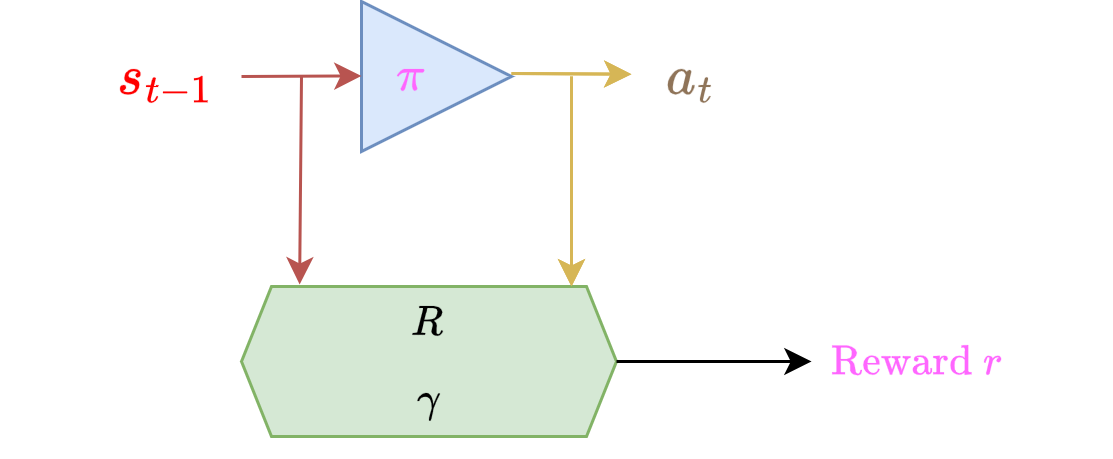
\includegraphics[width=90mm,scale=0.5]{images/mdp_images/policy_reward.png}
            
            \caption*{Our reward is based on the input/output of our policy: it can be seen as directly "observing" our policy function.}
        \end{figure}

        \begin{concept}
            While our value function $V_{\grn{\pi}}\big(\red{s} \big)$ only directly depends on $\pi$ and $s$, there's information we need from the MDP itself:
            
            \begin{itemize}
                \item The \purp{reward function} $\pur{R} \Big( \red{s},\bro{a} \Big)$: our average reward is made up of many individual rewards, for different situations.
                \item The \gren{transition function} $\grn{T} \Big( \red{s},\bro{a},\pur{s'} \Big)$: we need to know how likely different outcomes are, for our average.
            \end{itemize}

            In other words: our value function is specific to our MDP: two different MDPs will have completely separate value functions.
        \end{concept}

        Lastly, how we compute our value function depends on whether we're using \gren{finite} or \purp{infinite} horizon.


    \pagebreak

    \subsection{Finite Horizon}

        For our first setting, we'll assume that we are going to run our MDP for a precise length of \gren{time}, $h$. 
        
        \begin{itemize}
            \item This is our \vocab{horizon}: it tells us how "far away" the end of our MDP run is.

            \item After that time, we don't do anything with our MDP: no actions, no state changes, no rewards.\\
        \end{itemize}

        \begin{definition}
            The \vocab{horizon} $h$ of our MDP is the number of timesteps until it \purp{terminates}.

            Upon each \gren{timestep} $t$, our policy $\pi$ chooses an \brow{action $a_t$}, and our state machine transitions to \redd{state $s_t$}. Then, $t$ increases to $t+1$, and $h$ \textbf{decreases} to $h-1$.

            \begin{itemize}
                \item When our MDP terminates, we \purp{stop} taking actions, or receiving any reward.
                \item If \gren{$h=0$}, our MDP has already terminated: we can't take any more actions.
            \end{itemize}
        \end{definition}

        We can run our MDP as pseudocode, with MDP functions already defined:
            \note{Meaning, we've defined $f_s$ and $R$ already.}

        \begin{codebox}
            \Procname{$\proc{MDP\_Run}
                       (H, s_0, \pi)$}

                \li $h=H$ \qquad \qquad \#$H$ is the initial horizon
                
                \li $t=0$

                \li
                
                \li \While $h>0$  \qquad \qquad \#Not yet terminated
                    \Do
                        \li $\bro{a_t} = \grn{\pi}\big(\red{s_t}\big)$ \qquad \qquad \#Choose action
                        \li $\red{s_{t+1}} = \grn{f_s}\Big(\red{s_t},\bro{a_t}\Big)$ \qquad \qquad \#Next state based on $f_s$, described by $T$
                        \li
                        
                        \li \textbf{yield} $\pur{R}\Big(\red{s_t},\bro{a_t}\Big)$ \qquad \qquad \#New reward
                        \li
                        
                        \li $h=h-1$ \qquad \qquad \#Update horizon
                        \li $t=t+1$
                    \End

                \li
                \li \textbf{yield} \org{None} \qquad \qquad \#$h=0$, Program terminated
                       
        \end{codebox}

        Note that horizon goes down, and time goes up.\\

        \begin{clarification}
            $t$ indicates the \orgg{number of timesteps} since \purp{initialization} (the start of the MDP).

            $h$ indicates the \orgg{number of timesteps} until \gren{termination} (the end of the MDP).

            \begin{itemize}
                \item $t$ increases, while $h$ decreases, as our MDP runs.
            \end{itemize}
        \end{clarification}

        Because our horizon is a finite, natural number $h \in \NN$, we call this the \vocab{finite horizon} case.\\

        \begin{definition}
            If $h \in \NN$, then we are dealing with a \vocab{finite horizon problem}.
        \end{definition}

        


    \phantom{}

    \subsection{Finite Horizon Value Function}

        Now, we've set up the problem. In this \gren{finite-horizon} setting, we need to compute the value of different policies.

        The first thing to address: we now have a third variable in our value function: \purp{horizon}.

        \begin{itemize}
            \item The amount of \gren{time} remaining affects the total amount of rewards you can receive.
            \item \miniex If a button gives you 10 dollars, it's more valuable to be able to press it 5 times ($h=5$) than only 2 times ($h=2$).\\
        \end{itemize}

        \begin{definition}
            Your \vocab{finite-horizon value function} depends on three factors: \redd{current state}, \gren{policy}, and \purp{horizon}.
            

            We notate this combination as $V_{\grn{policy}}^{\pur{horizon}} \big(\red{state} \big)$. Typically, we write

            \begin{equation*}
                V_{\grn{\pi}}^{\pur{h}}\big(\red{s} \big)
            \end{equation*}

            This is our function is $V_{\grn{\pi}}^{\pur{h}}$, taking $\red{s}$ as an input.
            \begin{itemize}
                \item Each horizon-policy combination has its own function.
            \end{itemize}

            We'll use \orgg{function} notation again: it's the same as without horizon.

            \begin{equation*}
                V_{\grn{\pi}}^{\pur{h}} : \red{\mathcal{S}} \to \RR
            \end{equation*}

            
        \end{definition}

        How do we get started? This is actually pretty complicated:

        \begin{itemize}
            \item Suppose you have $h=5$, and there are \gren{three} possible options for your next state.
            \item Then, there are three possible options for the state after that. This \purp{repeats} until $h=0$.
            \item We have $3^5=243$ different possible outcomes, each with their own \gren{rewards}, and \purp{probability} of occurring.
        \end{itemize}

        Needless to say, it would be a massive headache to compute all of these possible outcomes at once, especially as $h$ gets larger.\\

        \begin{concept}
            Because MDPs are \purp{stochastic}, they can take many possible paths, even with the same starting state $s$, and same policy $\pi$.

            Computing every possible outcome directly can become very \orgg{expensive}.
        \end{concept}

        Instead, let's try a different tactic: we'll think of the simplest example possible. What would that be? $h=0$.

        \begin{itemize}
            \item When $h=0$, there are no further actions to be taken, and no more rewards.
            \item So, the expected reward is 0.\\
        \end{itemize}

        \begin{kequation}
            The total reward for a horizon-0 MDP is always 0, no matter what.

            \begin{equation*}
                V_{\grn{\pi}}^{\pur{0}}\big(\red{s} \big) = 0
            \end{equation*}
        \end{kequation}



    \phantom{}

    \subsection{Finite Horizon, $H=1$}

        We've gotten a start. Now let's try the \textit{second} simplest example, $H=1$. We have two stages:

        \begin{itemize}
            \item When $h=1$, we take exactly \purp{one} action, and get \purp{one} reward. 
            \item After that, $h=0$, and we're in the same situation as before: \redd{no more} rewards.
        \end{itemize}

        We'll break our problem into these two parts:

        \begin{equation}
            V_{\grn{\pi}}^{\pur{1}}\big(\red{s} \big) \quad=\quad 
            \Big(h=1 \text{ reward}\Big)
            + 
            \Big(h=0 \text{ reward}\Big)
        \end{equation}

        \begin{concept}
            After taking our first action at horizon $h$, we're in the \gren{same situation} as if we started in horizon $(h-1)$, with a new state $\blu{s'}$.

            Thus, we can \orgg{separate} the rewards for each timestep.
        \end{concept}

        We'll find the $h=1$ reward first.

        \begin{itemize}
            \item Our reward for each step is given by $\pur{R} \Big( \red{state},\bro{action} \Big)$.
            \item Our state is given by $\red{s}$. What about our action?
            \item Our \gren{policy} determines our action, based on our state: $\grn{\pi} \big(\red{s} \big)$.
        \end{itemize}

        \begin{equation}
            \Big(h=1 \text{ reward}\Big) \quad=\quad 
            \pur{R} \Big( \red{s},\grn{\pi}\big(\red{s}\big) \Big)
        \end{equation}

        This same reasoning works no matter which timestep you're starting on.\\

        \begin{concept}
            In our MDP, our \textbf{action} will always be determined by our \gren{policy}: 
            
            \begin{equation*}
                \bro{a} = \grn{\pi} \big(\red{s} \big)
            \end{equation*}

            Thus, our reward $\pur{R} \Big( \red{s},\bro{a} \Big)$ will always take the form

            \begin{equation*}
                \pur{R} \Big( \red{s},\grn{\pi}\big(\red{s}\big) \Big)
            \end{equation*}
        \end{concept}

        Now, the $h=0$ reward. We've moved into state $\blu{s'}$, but that doesn't matter: our reward is always 0.
            \note{At $h=1$, we gather our reward $\pur{R} \Big( \red{s},\grn{\pi}\big(\red{s}\big) \Big)$, but we also change states from $\red{s}$ to $\blu{s'}$.}

        \begin{equation}
            \Big(h=0 \text{ reward}\Big) \quad=\quad 
            V_{\grn{\pi}}^{\pur{0}}\big(\blu{s'} \big) 
            \quad=\quad 0
        \end{equation}
    
        Taken together, we get:

        \begin{equation}
            V_{\grn{\pi}}^{\pur{1}}\big(\red{s} \big) = 
            \overbrace{
                \pur{R} \Big( \red{s},\grn{\pi}\big(\red{s}\big) \Big)
            }^{h=1 \text{ reward}}
            + 
            \overbrace{
                V_{\grn{\pi}}^{\pur{0}}\big(\blu{s'} \big)
            }^{h=0 \text{ reward}}
        \end{equation}

        Or, 

        \begin{equation}
            V_{\grn{\pi}}^{\pur{1}}\big(\red{s} \big) = 
                \pur{R} \Big( \red{s},\grn{\pi}\big(\red{s}\big) \Big)
            + 
            0
        \end{equation}

        \begin{kequation}
            The total reward for a horizon-1 MDP equals the reward for taking one \redd{action}, according to \gren{policy}.
    
            \begin{equation*}
                V_{\grn{\pi}}^{\pur{1}}\big(\red{s} \big) = 
                    \pur{R} \Big( \red{s},\grn{\pi}\big(\red{s}\big) \Big)
            \end{equation*}
        \end{kequation}

        We can represent this similar to a state-transition diagram:
        
        \begin{figure}[H]
            \centering
            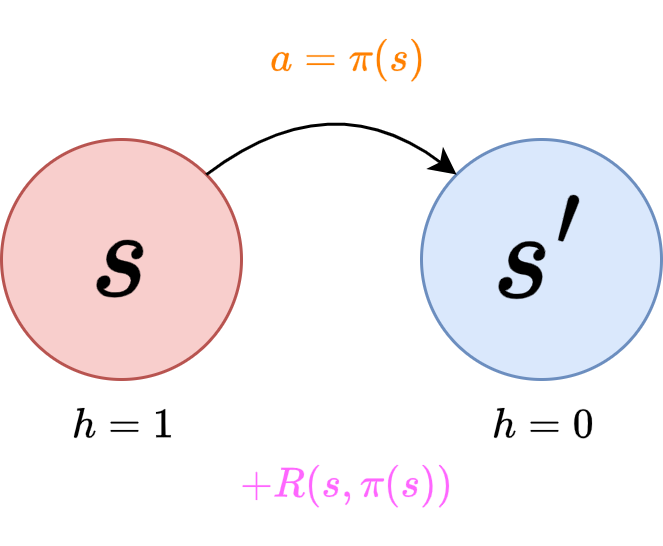
\includegraphics[width=40mm,scale=0.5]{images/mdp_images/horizon_1.png}
            
            \caption*{We take one action $\pi(s)$, and get a reward $R(s,a)$.}
        \end{figure}

        Note that, while we show only one future state $s'$, this is just one \textit{possible} outcome.
        \begin{itemize}
            \item You could think of this as one run of our MDP.
        \end{itemize}



    \phantom{}

    \subsection{Finite Horizon, $H=2$}

        Next, we'll tackle $H=2$. 

        \begin{itemize}
            \item When $h=2$, we take action $\grn{\pi}\big(\red{s}\big)$, moving from $\red{s}$ to $\blu{s'}$.
        
            \item When $h=1$, we take action $\grn{\pi}\big(\blu{s'}\big)$, moving from $\blu{s'}$ to $\pur{s''}$.
                \note{We already know $h=0$ gives \purp{no reward}.}
        \end{itemize}

        We can separate out the reward for each timestep:

        \begin{equation*}
            V_{\grn{\pi}}^{\pur{2}}\big(\red{s} \big) \quad=\quad 
            \Big(h=2 \text{ reward}\Big)
            +
            \Big(h=1 \text{ reward}\Big)
            + 
            \Big(h=0 \text{ reward}\Big)
        \end{equation*}

        And remove $h=0$:

        \begin{equation*}
            V_{\grn{\pi}}^{\pur{2}}\big(\red{s} \big) \quad=\quad 
            \Big(h=2 \text{ reward}\Big)
            +
            \Big(h=1 \text{ reward}\Big)
        \end{equation*}

        \begin{figure}[H]
            \centering
            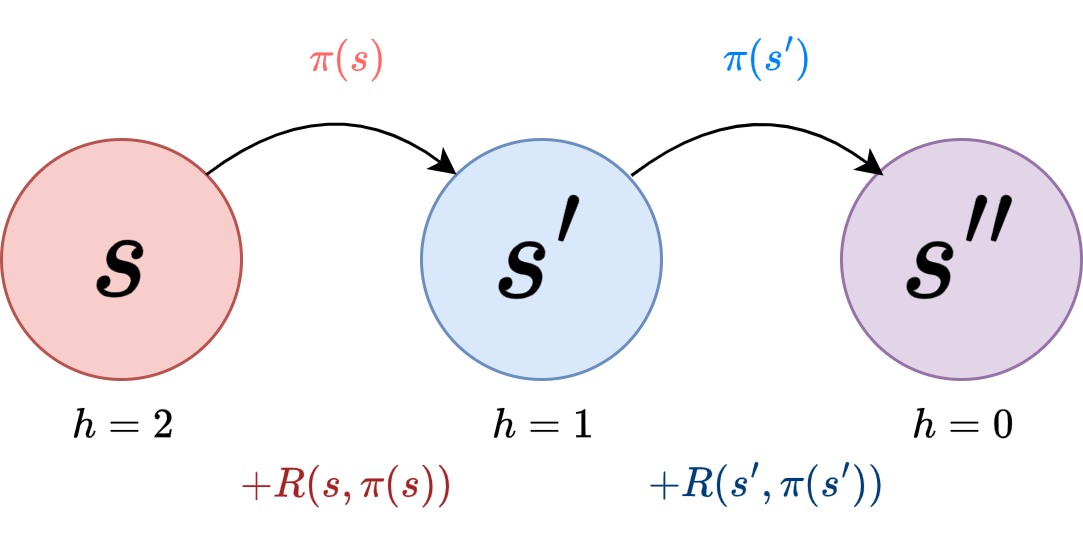
\includegraphics[width=70mm,scale=0.5]{images/mdp_images/horizon_2.png}
            
            \caption*{Two actions, two rewards.}
        \end{figure}

        \subsecdiv

        First, we'll compute the $h=2$ reward.

        \begin{itemize}
            \item This is the same as the the $H=1$ problem: we start in state $\red{s}$, and take action $\grn{\pi}\big(\red{s}\big)$.
        \end{itemize}

        \begin{equation}
            \Big(h=2 \text{ reward}\Big) \quad=\quad 
            \pur{R} \Big( \red{s},\grn{\pi}\big(\red{s}\big) \Big)
        \end{equation}

        \subsecdiv

        Now, we want to compute the $h=1$ reward.

        \begin{itemize}
            \item After $h=2$, we've moved to state $\blu{s'}$. We try to do what we did before:
        \end{itemize}

        \begin{equation}
            \Big(h=1 \text{ reward}\Big) \quad=\quad 
            \pur{R} \Big( \blu{s'},\grn{\pi}\big(\blu{s'}\big) \Big) 
            \qquad \text{...Maybe?}
        \end{equation}

        But we have a serious problem: which state is $\blu{s'}$?\\

        \begin{concept}
            Our \gren{state transition} is \gren{probabilistic}.

            \begin{itemize}
                \item That means that there are \gren{several new states} $\blu{s'}$ we could transition to.
            \end{itemize}

            So, we can't just directly use $\pur{R} \Big( \blu{s'},\grn{\pi}\big(\blu{s'}\big) \Big)$: we don't know which $\blu{s'}$ will be, and thus our reward.
        \end{concept}

        In other words, the reward for $h=1$ will depend on the random outcome of our \orgg{transition function} $T$.

        How do we resolve this? The key is to remember that $V$ is computing \purp{average reward}: meaning, we'll average our reward over all possible transitions.

        A quick review on how to do that:\\

        \begin{concept}
            Suppose we have a \purp{random variable} $X$ with multiple possible outcomes $x_i$. We want to get the average, or \vocab{expected value} $\mathbb{E} \big[ X \big]$.

            \begin{itemize}
                \item The more \gren{likely} an outcome, the more it \textbf{contributes} to the average.
            \end{itemize}

            Thus, $\mathbb{E} \big[ X \big]$ is a \orgg{weighted average} of each outcome, \gren{times} its probability.

            \begin{equation*}
                \mathbb{E} \big[ X \big] = 
                    \overbrace{\sum_{i} }^{\text{All outcomes}} 
                    x_i \cdot P \big(x_i\big)
            \end{equation*}
            
        \end{concept}

        \miniex Suppose you're betting on something: there's a 60\% chance you make \$100, and a 40\% chance you lose \$40. The average earnings (average \purp{reward}) is:

        \begin{equation}
            \mathbb{E} \big[ X \big] = 
            \sum_{i}  
                x_i \cdot P \big(x_i\big)
            \qquad=\qquad
            0.6 * 100 - 0.4 * 40 = \red{44}
        \end{equation}

        Now, we have the tools we need to proceed.

        \subsecdiv

        Let's apply this averaging to our current situation:

        \begin{itemize}
            \item We want to get the average reward, $\pur{R} \Big( \blu{s'},\grn{\pi}\big(\blu{s'}\big) \Big)$.
            \item We'll average over possible states $\blu{s'}$.
        \end{itemize}

        \begin{equation}
            \Big(h=1 \text{ reward}\Big)  
            \quad=\quad 
            \underbrace{
                \sum_{\blu{s_i} \in \mathcal{S}}  
                    \;\;
                    \pur{R} \Big( \blu{s_i},\grn{\pi}\big(\blu{s_i}\big) \Big)
                    \;\cdot\; 
                    P \big( \blu{s'}=s_i\big)
            }_{\text{Averaging over possible transitions to $\blu{s_i}$}}
        \end{equation}

        What's our probability $ P \big( \blu{s'}=s_i\big)$?

        \begin{itemize}
            \item Probabilities are determined by our transition function $\grn{T} \Big( \red{s},\bro{a},\pur{s'} \Big)$.
            \item $\grn{T} \Big( \red{s},\grn{\pi}\big(\red{s}\big),\pur{s'} \Big)$ represents our transition from $h=2$ to $h=1$.
        \end{itemize}

        In this situation, $\grn{T} \Big( \red{s},\grn{\pi}\big(\red{s}\big),\blu{s_i} \Big)$ is "the probability of moving to state $\blu{s_i}$".
            \note{Because we already know our initial state $\red{s}$ and our policy $\grn{\pi}$.}

        \begin{equation}
            P \big( \blu{s'}=s_i\big) \quad = \quad
            \grn{T} \Big( \red{s},\grn{\pi}\big(\red{s}\big),\blu{s_i} \Big)
        \end{equation}

        \begin{equation}
            \Big(h=1 \text{ reward}\Big) 
            \quad=\quad 
            \sum_{\blu{s_i} \in \mathcal{S}}  
                \;\;
                \underbrace{
                    \grn{T} \Big( \red{s},\grn{\pi}\big(\red{s}\big),\blu{s_i} \Big)
                }_{\text{Chance of state $\blu{s_i}$}}
                \;\cdot\; 
                \underbrace{
                \pur{R} \Big( \blu{s_i},\grn{\pi}\big(\blu{s_i}\big) \Big)
                }_{\text{Reward for state $\blu{s_i}$}}
        \end{equation}

        \begin{kequation}
            Suppose you know the \redd{state} $\red{s}$ of your MDP at horizon $H$.
            
            \begin{itemize}
                \item You can compute the reward for the next timestep, horizon $H-1$, by \purp{averaging over} all of the possible state transitions, to each state $\blu{s'}$.
            \end{itemize}

            \begin{equation*}
            \Big( \big(h=H-1\big) \text{ reward}\Big) 
                \quad=\quad 
                \sum_{\blu{s'}}  
                    \;\;
                        \grn{T} \Big( \red{s},\grn{\pi}\big(\red{s}\big),\blu{s'} \Big)
                    \;\cdot\; 
                    \pur{R} \Big( \blu{s'},\grn{\pi}\big(\blu{s'}\big) \Big)
            \end{equation*}
        \end{kequation}

        \subsecdiv

        We can assemble our full solution:\\

        \begin{kequation}
            The total reward for a horizon-2 MDP adds two rewards:
            
            \begin{itemize}
                \item The reward for taking one \redd{action}, according to \gren{policy}.
                \item \purp{Average} of all possible outcomes, based on the result of the \gren{state transition}.
            \end{itemize}

            
            \begin{equation*}
                V_{\grn{\pi}}^{\pur{2}}\big(\red{s} \big) =\quad 
                \overbrace{
                    \pur{R} \Big( \red{s},\grn{\pi}\big(\red{s}\big) \Big)
                }^{h=2 \text{ reward}}
                \;\;+\;\;
                \overbrace{
                    \sum_{\blu{s'}}  
                    \;\;
                        \grn{T} \Big( \red{s},\grn{\pi}\big(\red{s}\big),\blu{s'} \Big)
                    \;\cdot\; 
                    \pur{R} \Big( \blu{s'},\grn{\pi}\big(\blu{s'}\big) \Big)
                }^{h=1 \text{ reward}}
            \end{equation*}
        \end{kequation}

        Without the annotations, we see:

        \begin{equation*}
            V_{\grn{\pi}}^{\pur{2}}\big(\red{s} \big) =\quad 
                \pur{R} \Big( \red{s},\grn{\pi}\big(\red{s}\big) \Big)
            \;\;+\;\;
                \sum_{\blu{s'}}  
                \;\;
                    \grn{T} \Big( \red{s},\grn{\pi}\big(\red{s}\big),\blu{s'} \Big)
                \;\cdot\; 
                \pur{R} \Big( \blu{s'},\grn{\pi}\big(\blu{s'}\big) \Big)
        \end{equation*}



    \phantom{}

    \subsection{Finite Horizon, $H=3$ and beyond}

        Finally, we tackle $H=3$. And with this step, we come up with a strategy for all finite horizons.

        \begin{itemize}
            \item For $h=3$, we start in state $\red{s}$, and use our policy to act.
            \item For $h=2$, our action depends on the state $\blu{s'}$ we end up in, \gren{stochastically}.
                \note{Remember: "stochastic" describes our random state transition, with known probabilities.}
                \begin{itemize}
                    \item The same is true for $h=1$: our action depends on the state $\pur{s''}$.
                        \note{$h=0$ gives \purp{no reward}.}
                \end{itemize}
            
        \end{itemize}

        \begin{figure}[H]
            \centering
            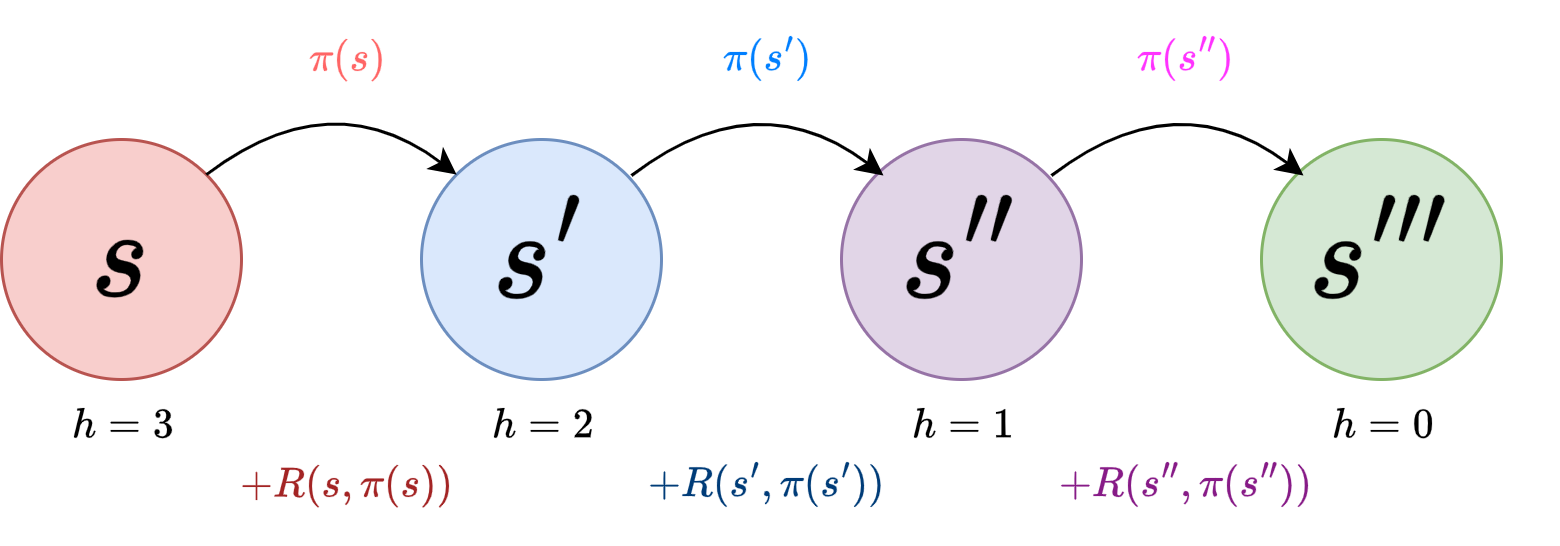
\includegraphics[width=90mm,scale=0.5]{images/mdp_images/horizon_3.png}
            
            \caption*{Three actions: $s'$ and $s''$ can vary based on our random transitions.}
        \end{figure}

        The reward for $h=3$ is the simplest: we know what \redd{state} we're in, and our policy's action. 

        What about $h=2$? Well, we could \purp{separately} get the reward for $h=2$, and $h=1$. But \textit{instead}, we'll consider the following:

        \begin{itemize}
            \item Suppose that we've already selected our new state, $\blu{s'}$. If we know our new state, this is \gren{identical} to the $H=2$ problem.\\
        \end{itemize}

        \begin{concept}
            If we know our \redd{current state}, we actually \purp{don't care} about what happened during earlier timesteps.

            \begin{itemize}
                \item That means, if our current horizon is $h=2$, we can pretend as if we're starting a new MDP run with $H=2$.
            \end{itemize}
        \end{concept}

        Let's forget $h=3$ for a moment:

        \begin{itemize}
            \item We're starting with $H=2$, from state $\blu{s'}$.
            \item We want to compute the total reward from this state, using our policy $\grn{\pi}$.
            \item We \purp{already computed} this above: the result is $V_{\grn{\pi}}^{\pur{2}}\big(\blu{s'} \big)$.\\
        \end{itemize}

        \begin{concept}
            $V_{\grn{\pi}}^{\pur{H}}\big(\blu{s'} \big)$ includes all the rewards for all timesteps between $h=H$ and $h=0$.

            \begin{equation*}
                V_{\grn{\pi}}^{\pur{H}}\big(\red{s} \big) \quad=\quad 
                \sum_{h=0}^{H} 
                \Big(\text{Immediate reward for horizon } h\Big)
            \end{equation*}

            Or,

            \begin{equation*}
                V_{\grn{\pi}}^{\pur{H}}\big(\red{s} \big) \quad=\quad 
                \Big( \text{Rewards for } h \leq H \Big)
            \end{equation*}

            That means, if we've already computed $V_{\grn{\pi}}^{\pur{H}}\big(\red{s}\big)$, it can handle the last $H$ steps of our MDP:

            \begin{equation*}
                V_{\grn{\pi}}^{\pur{H+1}}\big(\red{s} \big) \quad=\quad 
                \Big(\text{Reward for horizon } H+1 \Big)
                +
                \Big( \text{Rewards for } h \leq H \Big)
            \end{equation*}
        \end{concept}

        Remember to keep $V$ and $R$ separate in your mind:\\

        \begin{clarification}
            Our value function $V_{\grn{\pi}}^{\pur{h}}\big(\red{s} \big)$ gives us the \purp{expected reward for all current and future steps}, given a \redd{state} and \gren{policy}.

            Our reward function $\pur{R} \Big( \red{s},\grn{\pi}\big(\red{s}\big) \Big)$ gives us the \purp{reward for one step}, given a \redd{state} and \brow{action}.

        \end{clarification}

        \subsecdiv

        There's one important detail missing, though: this all assumes that we know $\blu{s'}$. But we don't, because of our random transitions.

        \begin{itemize}
            \item So, once again, we have to \purp{average} over all possible $\blu{s'}$.
        \end{itemize}

        \begin{equation}
            \Big( (h \leq H-1) \text{ rewards}\Big)  
            \quad=\quad 
                \sum_{\blu{s_i} \in \mathcal{S}}  
                    \;\;
                    P \big( \blu{s'}=s_i\big)
                    \;\cdot\; 
                    \overbrace{
                    V_{\grn{\pi}}^{\pur{H-1}}\big(\blu{s_i} \big)
                    }^{\text{Future rewards if }\blu{s'}=s_i}
        \end{equation}

        Again, we use our \gren{transition function}:

        

        \begin{equation}
            \Big( (h \leq H-1) \text{ rewards}\Big)    
            \quad=\quad 
                \sum_{\blu{s_i} \in \mathcal{S}}  
                    \;\;
                    \grn{T} \Big(          \red{s},\grn{\pi}\big(\red{s}\big),\blu{s'} \Big)
                    \;\cdot\; 
                    V_{\grn{\pi}}^{\pur{H-1}}\big(\blu{s_i} \big)
        \end{equation}

        \begin{concept}
            Often, we \redd{don't know} our next state, but we know the \purp{probability distribution} of states. 

            In this situation, we can:

            \begin{itemize}
                \item Use $\grn{T}$ to average all of our value functions, to get the \orgg{average future rewards}.
            \end{itemize}
        \end{concept}

        Now, we combine this with our first reward, for the initial $H$ step. Because we \gren{know} our state and policy, we don't have to use the transition function for our \purp{first} step.
            \note{This is always true for the $h=H$ step.}

        \begin{equation}
            \Big( (h \leq H) \text{ rewards}\Big) \;=\;
            \Big( (h = H) \text{ reward}\Big) +
            \Big( (h \leq H-1) \text{ rewards}\Big)
        \end{equation}

        \begin{equation}
            V_{\grn{\pi}}^{\pur{H}}\big(\red{s} \big) \;\;=\;\; \pur{R} \Big( \red{s},\grn{\pi}\big(\red{s}\big) \Big) +
            \sum_{\blu{s_i} \in \mathcal{S}}  
                    \;\;
                    \grn{T} \Big(          \red{s},\grn{\pi}\big(\red{s}\big),\blu{s_i} \Big)
                    \;\cdot\; 
                    V_{\grn{\pi}}^{\pur{H-1}}\big(\blu{s_i} \big)
        \end{equation}

        If we apply this to our $H=3$ example, we get:

        \begin{equation}
            V_{\grn{\pi}}^{\pur{3}}\big(\red{s} \big) \;\;=\;\; \pur{R} \Big( \red{s},\grn{\pi}\big(\red{s}\big) \Big) +
            \sum_{\blu{s_i} \in \mathcal{S}}  
                    \;\;
                    \grn{T} \Big(          \red{s},\grn{\pi}\big(\red{s}\big),\blu{s_i} \Big)
                    \;\cdot\; 
                    V_{\grn{\pi}}^{\pur{2}}\big(\blu{s_i} \big)
        \end{equation}

        \begin{kequation}
            The total reward for a horizon-$H$ MDP $V_{\grn{\pi}}^{\pur{H}}\big(\blu{s_i} \big)$ is broken into two parts:

            \begin{itemize}
                \item The reward for our \brow{first action}.
                \item The reward for \purp{all future steps}, based on the \gren{first transition} $\red{s}\to\blu{s'}$.
                    \begin{itemize}
                        \item The "all future steps" reward has already been computed for the \orgg{horizon-$(H-1)$} MDP, $V_{\grn{\pi}}^{\pur{H-1}}\big(\blu{s'} \big)$.
                        \item We'll average over each possible "first transition".
                    \end{itemize}
            \end{itemize}

            \begin{equation*}
                V_{\grn{\pi}}^{\pur{H}}\big(\red{s} \big) \;\;=\;\; 
                \overbrace{
                    \pur{R} \Big( \red{s},\grn{\pi}\big(\red{s}\big) \Big)
                }^{\text{First reward}} 
                \quad+\quad
                \overbrace{
                \sum_{\blu{s'}}  
                        \;\;
                        \underbrace{
                            \grn{T} \Big(   
                            \red{s},\grn{\pi}\big(\red{s}\big),\blu{s'} \Big)
                        }_{\text{Chance of } \red{s} \to \blu{s'}}
                        \;\;\; \cdot \;\;\; 
                        \underbrace{
                            V_{\grn{\pi}}^{\pur{H-1}}\big(\blu{s'} \big)
                        }_{\text{Reward if } \red{s} \to \blu{s'}}
                }^{\text{Future rewards}}
            \end{equation*}
        \end{kequation}

        If we remove the clutter, our equation is:

        \begin{equation}
            V_{\grn{\pi}}^{\pur{H}}\big(\red{s} \big) \;\;=\;\; 
                \pur{R} \Big( \red{s},\grn{\pi}\big(\red{s}\big) \Big) +
            \sum_{\blu{s'}}  
                    \;\;
                    \grn{T} \Big(          \red{s},\grn{\pi}\big(\red{s}\big),\blu{s'} \Big)
                    \;\cdot\; 
                    V_{\grn{\pi}}^{\pur{H-1}}\big(\blu{s'} \big)
        \end{equation}

    \pagebreak

    \subsection{Finite Horizon MDP Solution}

        We've created a general solution:

        \begin{itemize}
            \item If $H=0$, the reward is 0.
            \item If $H>0$, then we \orgg{break} the reward into two parts:
                \begin{itemize}
                    \item The \gren{immediate} reward
                    \item The \purp{future} rewards, based on the $H-1$ case.
                \end{itemize}
        \end{itemize}

        Since horizon $H$ depends on horizon $H-1$, we typically "\vocab{build up}" our solution, starting from $H=1$: 

        \begin{itemize}
            \item We compute $V_{\grn{\pi}}^{\pur{H}}$, and then $V_{\grn{\pi}}^{\pur{H+1}}$, gradually increasing horizon $H$.

            \item That way, when we do horizon $H$, we already have the \purp{value functions} we need (from $H-1$).
        \end{itemize}

        Let's show this gradual progression:

        \begin{equation}
            \org{V_{\pi}^{0}\big(s \big)}  \;\;=\;\; 
            0
        \end{equation}

        \begin{equation}
            \pur{V_{\pi}^{1}\big(s \big)} \;\;=\;\; 
                    R \Big( s,\pi\big(s\big) \Big)
                + \org{0}
        \end{equation}

        \begin{equation}
            \red{V_{\pi}^{2}\big(s \big)} \;\;=\;\; 
                    R \Big( s,\pi\big(s\big) \Big)
                +
                    \pur{\sum_{s'}}  
                        \;\;
                        T \Big(          s,\pi\big(s\big),s' \Big)
                        \;\cdot\; 
                        \pur{V_{\pi}^{1}\big(s' \big)}
        \end{equation}

        And if we keep going...

        \begin{equation}
            \grn{V_{\pi}^{H}\big(s \big)} \;\;=\;\; 
                    R \Big( s,\pi\big(s\big) \Big)
                +
                    \red{\sum_{s'}}  
                        \;\;
                        T \Big(          s,\pi\big(s\big),s' \Big)
                        \;\cdot\; 
                        \red{V_{\pi}^{H-1}\big(s' \big)}
        \end{equation}

        \begin{definition}
            Here, we present the equations for computing the \purp{value functions} for a \vocab{finite-horizon MDP}:

            \begin{equation*}
                V_{\grn{\pi}}^{\pur{0}}\big(\red{s} \big) \;\;=\;\; 
                0
            \end{equation*}

            \begin{equation*}
                V_{\grn{\pi}}^{\pur{H}}\big(\red{s} \big) \;\;=\;\; 
                        \pur{R} \Big( \red{s},\grn{\pi}\big(\red{s}\big) \Big)
                    +
                        \sum_{\blu{s'}}  
                            \;\;
                            \grn{T} \Big(          \red{s},\grn{\pi}\big(\red{s}\big),\blu{s'} \Big)
                            \;\cdot\; 
                            V_{\grn{\pi}}^{\pur{H-1}}\big(\blu{s'} \big)
            \end{equation*}

            We start by computing $V_{\grn{\pi}}^{\pur{1}}\big(\red{s} \big)$, then $V_{\grn{\pi}}^{\pur{2}}\big(\red{s} \big)$, and so on, incrementing our horizon each time.

            \begin{itemize}
                \item And at each step, we use the previous value function.
            \end{itemize}
        \end{definition}

        Once we know how to compute the value function for horizon $h$, we can compare different policies:\\

        \begin{concept}
            Suppose we have a given horizon $h$.

            If policy $\grn{\pi_1}$ is \orgg{better than} $\grn{\pi_2}$, then:

            \begin{itemize}
                \item For every state $\red{s}$, $\grn{\pi_1}$ is at least as good as $\grn{\pi_2}$.
                    \begin{equation*}
                        \forall \red{s \in \mathcal{S}}: \qquad \qquad
                        V_{\grn{\pi_1}}^{\pur{h}}\big(\red{s} \big)
                        \geq 
                        V_{\grn{\pi_2}}^{\pur{h}}\big(\red{s} \big)
                    \end{equation*}

                \item There is at least one state $\red{\hat{s}}$ where $\grn{\pi_1}$ is better than $\grn{\pi_2}$.

                    \begin{equation*}
                        \exists \red{\hat{s} \in \mathcal{S}}: \qquad \qquad
                        V_{\grn{\pi_1}}^{\pur{h}}\big(\red{\hat{s}} \big)
                        >
                        V_{\grn{\pi_2}}^{\pur{h}}\big(\red{\hat{s}} \big)
                    \end{equation*}
            \end{itemize}

            In other words: "$\grn{\pi_1}$ is always at least as good as $\grn{\pi_2}$, and sometimes better".
        \end{concept}

        \note{$\forall$ just means "for all / every", while $\exists$ means "there is at least one".}





        \pagebreak


        \subsection{Finite-Horizon, using our Blanket Example (\redd{Optional})}

        \miniex We can apply this to our blanket problem. 

        First, our transitions:

        \begin{figure}[H]
            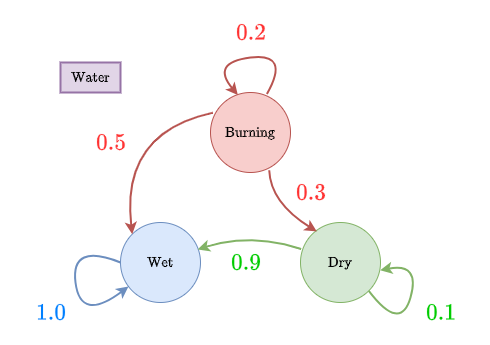
\includegraphics[width=80mm,scale=0.4]{images/mdp_images/add_water_transition.png}
            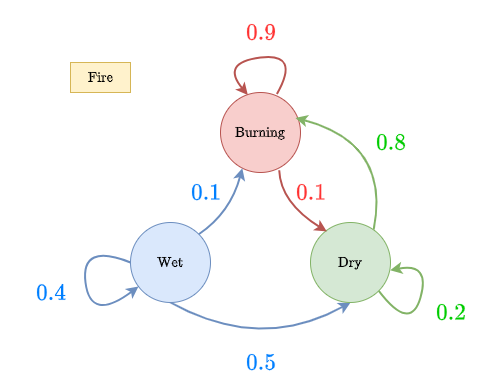
\includegraphics[width=80mm,scale=0.4]{images/mdp_images/add_fire_transition.png}
        \end{figure}

        Now, our rewards:

        \begin{equation}
            \pur{R} \Big( \red{s},\bro{a} \Big) =
            \begin{cases}
                10 & \red{s} = \text{Dry} \\
                0 & \red{s} = \text{Wet} \\
                -20 & \red{s} = \text{Burning}
            \end{cases}
        \end{equation}

        Finally, our policy:

        \begin{equation}
            \pi \big( \red{s} \big) =
            \begin{cases}
                \text{\brow{Add fire}} & s = \red{Wet} \\
                \text{\brow{Add water}} & s = \red{Dry} \\
                \text{\brow{Add water}} & s = \red{Burning}
            \end{cases}
        \end{equation}

        We have 3 states: 3 value functions for each horizon $h$.\\

        \begin{notation}
            Often, it's easier to write each \vocab{value function} in a \purp{condensed} form, to make equations easier to read.

            \begin{itemize}
                \item This is best used for your personal calculations: you need to be clear about what system you're using to \gren{abbreviate}.
            \end{itemize}

            In this case, we'll use:

            \begin{equation*}
                V_{\grn{\pi}}^h\big(\red{Dry}\big) = d_h
                \qquad
                V_{\grn{\pi}}^h\big(\red{Wet}\big) = w_h
                \qquad
                V_{\grn{\pi}}^h\big(\red{Burning}\big) = b_h
            \end{equation*}
        \end{notation}

        \subsecdiv

        The reward for $h=0$ is 0, no matter our state.

        \begin{equation}
            d_0=0 \qquad w_0 = 0 \qquad b_0 = 0
        \end{equation}

        \subsecdiv

        The reward for $h=1$ uses the formula
            \note{This is a simplified version of our general equation: because $V_{\grn{\pi}}^{\pur{0}}\big(\red{s} \big)=0$, the future steps can be skipped.}

        \begin{equation*}
            V_{\grn{\pi}}^{\pur{1}}\big(\red{s} \big) = 
                \pur{R} \Big( \red{s},\grn{\pi}\big(\red{s}\big) \Big)
        \end{equation*}

        Our immediate reward is only based on our current state, according to $\pur{R} \Big( \red{s},\bro{a} \Big)$.

        \begin{equation}
            d_1 = 10 \qquad w_1 = 0 \qquad b_1 = -20
        \end{equation}

        \subsecdiv

            For $h=2$, we have to use our general formula

            \begin{equation*}
                V_{\grn{\pi}}^{\pur{H}}\big(\red{s} \big) \;\;=\;\; 
                        \pur{R} \Big( \red{s},\grn{\pi}\big(\red{s}\big) \Big)
                    +
                        \sum_{\blu{s'}}  
                            \;\;
                            \grn{T} \Big(          \red{s},\grn{\pi}\big(\red{s}\big),\blu{s'} \Big)
                            \;\cdot\; 
                            V_{\grn{\pi}}^{\pur{H-1}}\big(\blu{s'} \big)
            \end{equation*}

        \begin{itemize}
            \item If it's dry, add water.

        \begin{equation}
            d_2 =  
            \overbrace{10}^{R_d} +  
            \overbrace{
            \Big(
                0.1 d_1 + 
                0.9 w_1
            \Big)
            }^{\sum_{\blu{s'}}  
                \grn{T}(...)
                V_{\grn{\pi}}^1(\blu{s'} )}
            \quad = \quad
            \org{11}
        \end{equation}
        
        
        \item If it's wet, add fire.
        
        \begin{equation}
            w_2 = 
            \overbrace{0}^{R_w} + 
            \overbrace{
            \Big(
                0.5d_1 + 0.4w_1 + 0.1b_1
            \Big)
            }^{\sum_{\blu{s'}}  
                \grn{T}(...)
                V_{\grn{\pi}}^1(\blu{s'} )}
            \quad=\quad
            \org{3}
        \end{equation}

        \item If it's burning, add water.

        \begin{equation}
            b_2 = 
            \overbrace{-20}^{R_b} +  
            \overbrace{
            \Big(
                0.3d_1+0.5w_1+0.2b_1
            \Big)
            }^{\sum_{\blu{s'}}  
                \grn{T}(...)
                V_{\grn{\pi}}^1(\blu{s'} )}
            \quad=\quad
            \org{-21}
        \end{equation}

        \end{itemize}

        We can repeat this process, with the same equations, for \gren{larger and larger} horizons, up to any particular $h$.




        

    \pagebreak

    \subsection{Infinite Horizon}

        In finite horizon, we knew exactly how long our MDP would run for.
        
        \begin{itemize}
            \item But often, we don't know how long it'll run for: or at the very least, it'll be a \gren{very long time}.
        \end{itemize}

        So, we'll consider an \purp{infinite horizon}:\\

        \begin{definition}
            In the \vocab{infinite horizon problem}, we \orgg{don't know} how long our MDP will run: it can run for a long time.
        \end{definition}

        In this situation, our horizon \purp{never changes}: if you take $n$ steps, you still don't know when the MDP will end.
            \note{We call this "infinite" because we've moved our 100\% certain \gren{horizon} infinitely far away.}
 

        \begin{figure}[H]
            \centering
            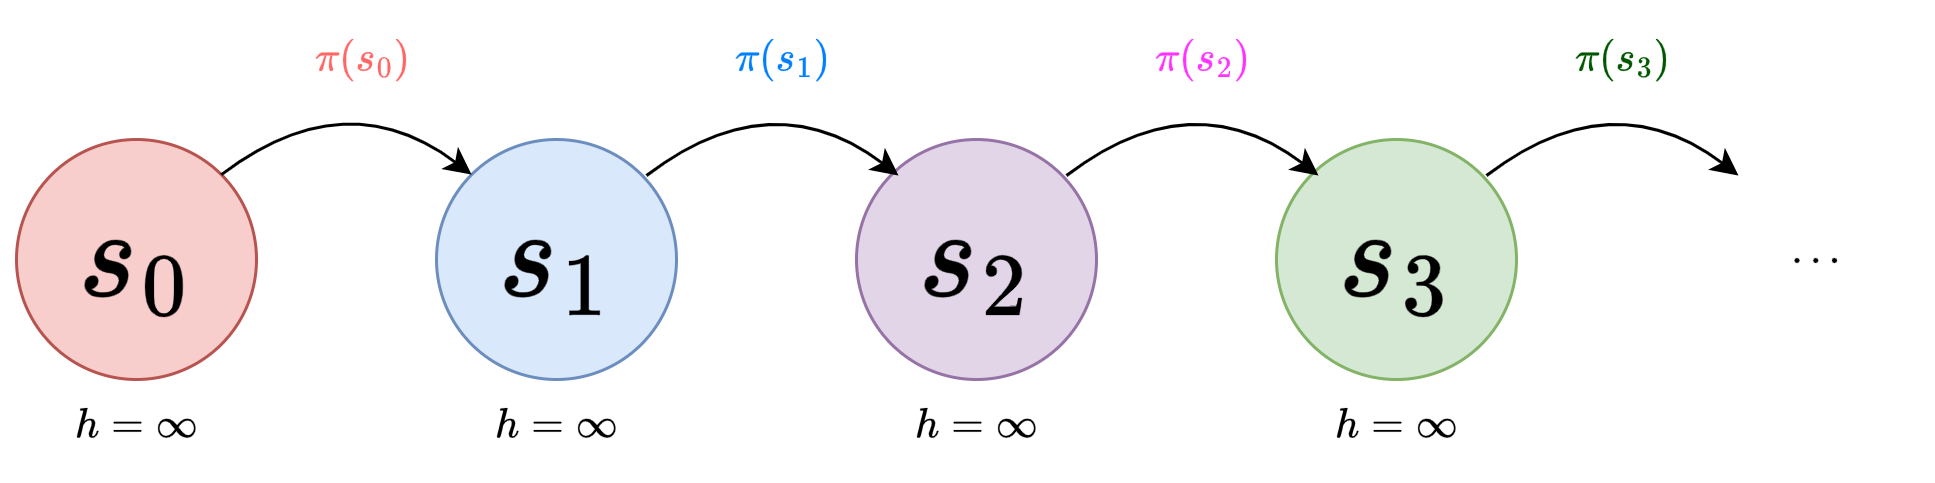
\includegraphics[width=100mm,scale=0.5]{images/mdp_images/infinite_horizon.png}
            
            \caption*{No matter how many steps we take, the horizon is always the same.}
        \end{figure}

        So, we don't use it as a variable.\\

        \begin{definition}
            Our \vocab{infinite-horizon value function} $V_{\grn{\pi}}^{\infty}$ doesn't require a horizon, because it's always the same. 

            This value function behaves the same as before: input is state $\red{s}$, output is \gren{average reward} $r$.

            \begin{equation*}
                V_{\grn{\pi}}^{\infty} : \red{\mathcal{S}} \to \RR
            \end{equation*}
        \end{definition}

        Note:\\

        \begin{notation}
            We can notate our \vocab{infinite-horizon value function} two ways:

            \begin{equation*}
                V_{\grn{\pi}}^{\infty}\big(\red{s} \big) = 
                V_{\grn{\pi}}\big(\red{s} \big)
            \end{equation*}

            For readability, we'll use $V_{\grn{\pi}}\big(\red{s} \big)$ in following sections.
        \end{notation}



    \phantom{}

    

    \subsection{Discounting}



        This model has a major bug we need to work out: infinite rewards.\\

        \begin{concept}
            If we run our MDP for an "infinite" amount of time, it can get an \purp{infinite} amount of \purp{rewards}.

            This makes it difficult to \gren{compare} two different policies that both have infinite value.
        \end{concept}

        \miniex Imagine you have two policies: one presses the "earn \$10" button, and the other presses the "earn \$20" button.

        \begin{itemize}
            \item Over an infinite timescale, both policies have a value of $\infty$, even though one is obviously better.
        \end{itemize}

        Our solution is to consider the \vocab{discounted infinite horizon}: we treat future rewards as less valuable ("discounted") than present rewards. 
        
        This brings us back to our $\gamma$ factor from the beginning of the chapter:\\

        \begin{definition}
            $\pur{\gamma}$ is our \purp{discount factor}, which tells us how much we value future rewards.

            \begin{equation*}
                \gamma \in \Big[ 0,1 \Big]
            \end{equation*}

            The \gren{higher} $\gamma$ is, the \gren{more} we value future rewards.

            \begin{itemize}
                \item A reward $t$ timesteps in the future, is worth $\gamma^t$ times as much.
            \end{itemize}

            \subsecdiv

            Because $\gamma$ is never larger than 1, our discount factor can only either:

            \begin{itemize}
                \item Treat future rewards as \purp{equal} to current rewards ($\gamma=1$, \orgg{finite horizon})

                \item Treat future rewards as \purp{lesser} than current rewards ($\gamma<1$, \orgg{infinite horizon})
            \end{itemize}
        \end{definition}

        \miniex We'll re-use the above example, and use $\gamma=0.9$. 
        
        \begin{itemize}
            \item So, for each timestep, we scale down the reward by $0.9^{t}$.
                \note{For simplicity, our first timestep is $t=0$, not $t=1$.}
        \end{itemize}

        If we have the same reward $r$ for every time step, we get:
            \note{This is a geometric sum!}

        \begin{equation}
            V_{\grn{\pi}}\big(\red{s} \big) = r+ r\gamma + r\gamma^2+\cdots \qquad=\qquad r \sum_{t=0}^\infty \gamma^t = \frac{r}{1-\gamma}
        \end{equation}

        Let's compare our \$20 button to our \$10 button. 

        \begin{equation}
            V_{\grn{\$10}}\big(\red{s} \big) = 100 \qquad 
            V_{\grn{\$20}}\big(\red{s} \big) = 200
        \end{equation}

        Now, it's clear which policy is better.\\

        \begin{definition}
            For finite horizon, our value function is given by the \vocab{average total rewards}.

            \begin{equation*}
                V_{\grn{\pi}}^{h}\big(\red{s} \big)
                =
                \mathbb{E} \Big[\;\;
                    \sum_{t=1}^h R_t
                \;\;\Big]
            \end{equation*}

            For infinite horizon, our value function is given by the \vocab{average discounted rewards}.

            \begin{equation*}
                V_{\grn{\pi}}\big(\red{s} \big)
                =
                \mathbb{E} \Big[\;\;
                    \sum_{t=1}^h \gamma^t R_t
                \;\;\Big]
            \end{equation*}

            \subsecdiv

            In both cases, $R_t$ is based on our \redd{state} and \gren{policy}. 
        \end{definition}

            \note{Remember that $\mathbb{E} \Big[\cdot \Big]$ gives our average, or \purp{expected value}.} 

        There are a few justifications for why we could discount future value:

        \begin{itemize}
            \item Economics: \gren{money} is worth more now than in the future.
            \item Predictability: in the real world, it's harder to accurately predict the distant future than near future: distant rewards are thus less reliable/valuable.
        \end{itemize}

    \subsection{Discount factor: Termination}

        One of the most useful interpretations is \orgg{termination}: 

        We call our horizon "infinite", meaning that we don't have a \purp{definite stopping point} $h=0$ for our MDP.
        
        \begin{itemize}
            \item But, that \textit{doesn't} mean it never terminates: we just don't know \gren{when}.
        \end{itemize}

        Instead, consider this: at every timestep, our MDP has a \gren{$(1-\gamma)$} chance of terminating. We can only get our \purp{reward} if it \textbf{doesn't terminate}: probability $\gamma$.

        \begin{itemize}

            \item The chance of our model surviving for $t$ timesteps, and thus receiving reward $R_t$, is \red{$\gamma^t$}.\\
        \end{itemize}

        \begin{concept}
            We can interpret our infinite-horizon MDP having an "opportunity" to fail("terminate"), after every timestep.
            
            \begin{itemize}
                \item Our \vocab{discount factor} $\gamma$ is the chance of our MDP \gren{continuing}.
                \item $1-\gamma$ is the chance of our MDP \purp{terminating}.
            \end{itemize}

            So, while our MDP is unlikely to run "forever", there's no fixed horizon $h$ that it will \textit{definitely} terminate at.
        \end{concept}

        This is why we scale down our reward for $R_t$ by a factor of $\gamma^t$: because we're computing \purp{expected reward}.

        \begin{equation}
            \mathbb{E}\Big[ r_t  \Big] = 
            \overbrace{\grn{\gamma^t} \cdot R_t}^{\text{Model continues}} + 
            \overbrace{\red{(1-\gamma^t)} \cdot 0}^{\text{Model terminates}}
        \end{equation}

        \begin{itemize}
            \item Note that we can "miss" the reward for $R_t$ by failing at \purp{any step} before $t$. 
                \note{Make sure not to confuse $(1-\gamma^t)$ with $(1-\gamma)^t$: compare \textbf{exponents}.}
        \end{itemize}

        If the model terminates, we get 0 reward. So, we can ignore that part of the reward.

        \begin{equation}
            \mathbb{E}\Big[ r_t  \Big] = 
            \gamma^t \cdot R_t
        \end{equation}

        And this is how we get our $V_{\grn{\pi}}\big(\red{s} \big)$ expression above.

    \phantom{}

    \subsection{Lifespan of our MDP}

        As we mentioned, the horizon of our infinite-horizon model never changes.

        But we also find something more surprising: \purp{average future lifespan} (average number of timesteps until termination) is the \gren{exact same}, before and after one step.
            \note{We could think of this as the "average horizon": on average, how long does our MDP have left?}

        Let's find out why.

        \subsecdiv

        \miniex Suppose you're repeatedly flipping a fair coin. You count the number of tails you get. If you ever get heads, you \purp{stop playing}.
            \note{A "fair coin" is 50\% heads, 50\% tails.}

        Suppose you flip your coin once, and get tails. What are the odds of your next coin being heads?

        \begin{itemize}
            \item They're \gren{the same} as they were before that first coin toss: 50\%.
        \end{itemize}

        What if you flip your coin, and get 10 tails in a row?

        \begin{itemize}
            \item The odds of your next coin being heads is \orgg{still} 50\%.
        \end{itemize}

        \begin{concept}
            In an MDP, the \purp{odds of termination}, $(1-\gamma)$, are \gren{constant}.
        \end{concept}

        \subsecdiv

        We can apply this to the \purp{average amount of time left} until the model terminates.

        \begin{itemize}
            \item \miniex Suppose you just got 10 tails in a row. Technically speaking, the \gren{average remaining time} until the game ends is unchanged.
            \item The coin doesn't "\purp{remember}" that it just won 10 times: you have exactly the same coin as if you just started playing.
                \note{Consider the opposite case: if "winning 10 times" decreased the remaining time, that means that our coin is suddenly more likely to lose. Why would the coin change?}
        \end{itemize}

        We can describe this argument for all MDPs:

        \begin{itemize}
            \item This "average future lifespan" is based on the odds of termination at each turn.
            \item Since the odds of termination $\gamma$ are the same, the \purp{average future lifespan} is unchanged.\\
        \end{itemize}

        \begin{clarification}
            The fact that the \purp{average future lifespan} of our MDP is \gren{unchanged}, is often counter-intuitive.

            We'll address two points of confusion:

            \begin{itemize}
                \item As a real machine gets older, it's \purp{more likely} to break.
                
                \begin{itemize}
                    \item But that's because the odds of it breaking \gren{each day} are going up, because it wears out.
                    \item Nothing in our MDP is "\orgg{wearing out}": it just might spontaneously stop.
                \end{itemize}
                    
    
                \item It feels like the model should've "\purp{lost}" some of its life, after time passes. 

                    \begin{itemize}
                        \item This "lost" life is accounted for by the situation where the model immediately \redd{failed}.
                        \item What's changed about the situation is we know the model model \gren{succeeded}: we're biasing towards a longer total lifetime.
                    \end{itemize}
            \end{itemize}
        \end{clarification}

        So, your "average future lifespan" is the same, while your "average total lifespan" has increased by 1. 

        The "average future lifespan", by the way, is always $\frac{1}{1-\gamma}$. Why?

        \begin{itemize}
            \item $(1-\gamma)$ gives our failure odds.
            \item If the odds of something happening are $1/4$, you would \textbf{expect} to wait 4 times for it to happen.
                \note{It happens 1 in 4 times, after all.}
            \item So, you just take the \purp{reciprocal}.\\
        \end{itemize}

        \begin{kequation}
            The \vocab{average time until termination} ("average future lifespan") of our model is always 

            \begin{equation*}
                \frac{1}{1-\gamma}
            \end{equation*}
        \end{kequation}

        We always have the same horizon, and the same properties. This is a result of the \purp{markov property}:\\

        \begin{definition}
            MDPs are \vocab{memoryless}.

            \begin{itemize}
                \item \purp{Future states} are \gren{only} affected by the \textbf{current state and action}.

                \item Information in the \purp{past} has no effect: thus, our MDP doesn't have "memory" of these past events.
            \end{itemize}

            This is also called the \vocab{markov property}.

            \subsecdiv

            One effect of this property is that the \purp{average future lifespan} is \gren{always the same}.
        \end{definition}

        One more note:\\

        \begin{remark}
            Often, in probability, we're referring to a "\gren{weaker}" (having less requirements) version of \vocab{memorylessness}:

            \begin{itemize}
                \item It \redd{doesn't matter} how long we've been waiting for an event: the time until that event (waiting time) \purp{does not change}.
            \end{itemize}

            This is equivalent to the idea that "the \purp{average future  lifespan} never changes".
        \end{remark}

    \pagebreak

    \subsection{Infinite Horizon Value Function}

        Let's figure out our value function, starting from the finite horizon one:

        \begin{equation}
            V_{\grn{\pi}}^{\pur{H}}\big(\red{s} \big) \;\;=\;\; 
                \pur{R} \Big( \red{s},\grn{\pi}\big(\red{s}\big) \Big) +
            \sum_{\blu{s'}}  
                    \;\;
                    \grn{T} \Big(          \red{s},\grn{\pi}\big(\red{s}\big),\blu{s'} \Big)
                    \;\cdot\; 
                    V_{\grn{\pi}}^{\pur{H-1}}\big(\blu{s'} \big)
        \end{equation}

        First of all: our \purp{horizon never changes}: if our model didn't terminate, we're in the same situation after each timestep.\\

        \begin{concept}
            \orgg{Past events} do not matter to our \vocab{infinite-horizon MDP}.

            \begin{itemize}
                \item If we already survived $t$ timesteps in the \purp{past}, that has no effect on the odds of surviving in the \gren{future}.
                \item We're in the same situation as when we started.
            \end{itemize}

            
        \end{concept}

        \miniex Suppose that every round of a game, you \orgg{flip a coin} to decide whether you'll continue.

        \begin{itemize}
            \item Knowing that you've already survived 5 rounds has \gren{no effect} on how likely you are to survive the next round.
            \item We can \purp{ignore} those earlier rounds, and pretend as if we've just started playing.
        \end{itemize}

        This simplifies our work: we just remove the horizon. 

        \begin{equation}
            V_{\grn{\pi}}\big(\red{s} \big) \;\;=\;\; 
                \pur{R} \Big( \red{s},\grn{\pi}\big(\red{s}\big) \Big) +
            \sum_{\blu{s'}}  
                    \;\;
                    \grn{T} \Big(          \red{s},\grn{\pi}\big(\red{s}\big),\blu{s'} \Big)
                    \;\cdot\; 
                    V_{\grn{\pi}}\big(\blu{s'} \big)
            \qquad \quad (\text{if } \gamma=1)
        \end{equation}

        $V_{\grn{\pi}}\big(\blu{s'} \big)$ doesn't care how many rounds it's been since we started.

        \subsecdiv

        Now, we need to account for $\gamma$.

        Originally, we added $\grn{T}$ to represent the \purp{odds} of ending up in state $\blu{s'}$, and thus getting the reward from $V_{\grn{\pi}}\big(\blu{s'} \big)$.

        \begin{equation}
            \prob{\text{\blu{s'} reward} } = \grn{T} \Big(          \red{s},\grn{\pi}\big(\red{s}\big),\blu{s'} \Big)
        \end{equation}

        But that was when we knew that our model would continue. Now, we have to include two \purp{independent} events:

        \begin{itemize}
            \item We end up in state $\blu{s'}$: $\grn{T} \Big(          \red{s},\grn{\pi}\big(\red{s}\big),\blu{s'} \Big)$
            \item Our model doesn't \orgg{terminate} immediately: $\gamma$.
        \end{itemize}

        We just have to multiply these odds together.

        \begin{equation}
            \prob{\text{\blu{s'} reward} } = \overbrace{\gamma}^{\text{MDP doesn't terminate}} \cdot 
            \overbrace{
                \grn{T} \Big(          \red{s},\grn{\pi}\big(\red{s}\big),\blu{s'} \Big)
            }^{\text{End up in state } \blu{s'}}
        \end{equation}

        \begin{concept}
            In our \vocab{infinite MDP}, we have to include our $\gamma$ factor, \purp{diminishing} the value of future rewards by that factor.
        \end{concept}

        We get:

        \begin{equation}
            \grn{V_{\pi}\big(s \big)} \;\;=\;\; 
                    R \Big( s,\pi\big(s\big) \Big)
                +
                    \red{\sum_{s'}}  
                        \;\;
                        \blu{\gamma} \cdot 
                        T \Big(          s,\pi\big(s\big),s' \Big)
                        \;\cdot\; 
                        \grn{V_{\pi}\big(s' \big)}
        \end{equation}

        Or, we can even pull $\gamma$ out of the sum: all future rewards assumes the model doesn't terminate.\\

        \begin{kequation}
            We can compute the \vocab{infinite-horizon value function} using the following, \gren{recursive} equation.

                \begin{equation*}
                    V_{\grn{\pi}}\big(\red{s} \big) \;\;=\;\; 
                        \pur{R} \Big( \red{s},\grn{\pi}\big(\red{s}\big) \Big) +
                    \gamma
                    \sum_{\blu{s'}}  
                            \;\;
                            \grn{T} \Big(          \red{s},\grn{\pi}\big(\red{s}\big),\blu{s'} \Big)
                            \;\cdot\; 
                            V_{\grn{\pi}}\big(\blu{s'} \big)
                \end{equation*}
        \end{kequation}

            \note{We call it \gren{recursive} because $V_{\grn{\pi}}$ references itself in this equation.}



    \phantom{}


    

    \subsection{Solving the Infinite-Horizon Value Function}

        We can't solve this version like how we'd solve the \purp{finite-horizon} case: it doesn't make as much sense to do $h=1$, $h=2$, etc.

        But this version is, in some ways, \gren{simpler}: 

        \begin{itemize}
            \item The equation for $V_{\grn{\pi}}\big(\red{s}\big)$ contains other $V_{\grn{\pi}}$ functions.

            \item And we have one equation for each state $\red{s}$.
        \end{itemize}

        So, if we gather all of the equations for every $\red{s \in \mathcal{S}}$, we can \purp{solve} for each value function.
            \note{We're also in luck: our value function equations are \gren{linear!}}\\

        \begin{concept}
            In order to compute the \vocab{infinite-horizon value function} for every state, we can follow these steps:

            \begin{itemize}
                \item Write out the equation for value function $V_{\grn{\pi}}\big(\red{s}\big)$ for \redd{every state}, using the other value functions $V_{\grn{\pi}}\big(\blu{s'}\big)$.
                \item If we have $n$ states, we now have $n$ equations.
                \item Solve our $n$ \gren{equations} for our $n$ \gren{variables}, as a \purp{linear system}.
            \end{itemize}
        \end{concept}

            \note{The number of states is the same as the size of of our set $\mathcal{S}$. So, we can also write it as $n=|\mathcal{S}|$.}

        You can use any of our known tactics for solving linear systems.

    \pagebreak

    \subsection{Infinite-Horizon, using our Blanket Example (\redd{Optional})}

        \miniex We can apply this to our blanket problem. Let's set our discount factor at $\gamma=0.8$.

        First, our transitions:

        \begin{figure}[H]
            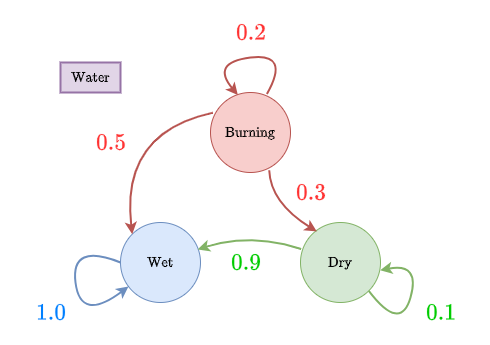
\includegraphics[width=80mm,scale=0.4]{images/mdp_images/add_water_transition.png}
            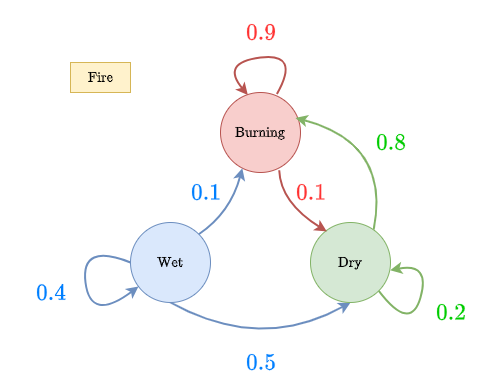
\includegraphics[width=80mm,scale=0.4]{images/mdp_images/add_fire_transition.png}
        \end{figure}

        Now, our rewards:

        \begin{equation}
            \pur{R} \Big( \red{s},\bro{a} \Big) =
            \begin{cases}
                10 & \red{s} = \text{Dry} \\
                0 & \red{s} = \text{Wet} \\
                -20 & \red{s} = \text{Burning}
            \end{cases}
        \end{equation}

        Finally, our policy:

        \begin{equation}
            \pi \big( \red{s} \big) =
            \begin{cases}
                \text{\brow{Add fire}} & s = \red{Wet} \\
                \text{\brow{Add water}} & s = \red{Dry} \\
                \text{\brow{Add water}} & s = \red{Burning}
            \end{cases}
        \end{equation}

        We want three value functions.\\

        \begin{notation}
            Often, it's easier to write each \vocab{value function} in a \purp{condensed} form, to make equations easier to read.

            \begin{itemize}
                \item This is best used for your personal calculations: you need to be clear about what system you're using to \gren{abbreviate}.
            \end{itemize}

            In this case, we'll use:

            \begin{equation*}
                V_{\grn{\pi}}\big(\red{Dry}\big) = d 
                \qquad
                V_{\grn{\pi}}\big(\red{Wet}\big) = w
                \qquad
                V_{\grn{\pi}}\big(\red{Burning}\big) = b
            \end{equation*}
        \end{notation}

        Let's get the equations for each value function.

        \begin{itemize}
            \item If it's dry, add water.
        

        \begin{equation}
            d = 
            \overbrace{10}^{R_d} + 
            \underbrace{0.8}_{\gamma} \cdot 
            \overbrace{
            \Big(
                0.1 d + 
                0.9 w
            \Big)
            }^{\sum_{\blu{s'}}  
                \grn{T}(...)
                V_{\grn{\pi}}(\blu{s'} )}
        \end{equation}
        
        \item If it's wet, add fire.
        
        \begin{equation}
            w = 
            \overbrace{0}^{R_w} + 
            \underbrace{0.8}_{\gamma} \cdot 
            \overbrace{
            \Big(
                0.5d + 0.4w + 0.1b
            \Big)
            }^{\sum_{\blu{s'}}  
                \grn{T}(...)
                V_{\grn{\pi}}(\blu{s'} )}
        \end{equation}

        \item If it's burning, add water.

        \begin{equation}
            b = 
            \overbrace{-20}^{R_b} + 
            \underbrace{0.8}_{\gamma} \cdot 
            \overbrace{
            \Big(
                0.3d+0.5w+0.2b
            \Big)
            }^{\sum_{\blu{s'}}  
                \grn{T}(...)
                V_{\grn{\pi}}(\blu{s'} )}
        \end{equation}

        \end{itemize}

        If we solve this \vocab{linear system}, we get:

        \begin{equation}
            \begin{matrix}
                d = V_{\grn{\pi}}\big(\red{Dry}\big) \approx 17.6\\
                w = V_{\grn{\pi}}\big(\red{Wet}\big) \approx 8.7\\
                b = V_{\grn{\pi}}\big(\red{Burning}\big) \approx -14.6\\
            \end{matrix}
        \end{equation}

        

        

